
\documentclass[%
paper=A4,               % Papiergröße
twoside=true,           % zweiseitiges Layout
openright,              % Kapitel auf ungerader Seite beginnen
11pt,                   % Schriftgröße
bibliography=totoc,     % Literaturverzeichnis im Inhaltsverzeichnis
%listof=totoc,           % Abb.-/Tab.-verzeichnis im Inhaltsverzeichnis
titlepage=on,           % Titel auf eigener Seite
DIV=12,                 % Satzspiegelberechnung
BCOR=1.5cm,             % Bindungskorrektur
parskip=half,            % Absatzabstand
final
]{scrreprt}
\usepackage{csquotes}
\usepackage[backend=biber, style=numeric, autocite=inline]{biblatex}
\usepackage[colorlinks]{hyperref}

\usepackage{enumitem}
\usepackage{setspace}
\usepackage{graphicx} 
\usepackage{float}
\usepackage{subcaption}



\hypersetup{
	citecolor=black,
	linkcolor=black,
	urlcolor=blue
}
\addbibresource{bachelorthesisSources.bib}

%Informationen zur Arbeit
\newcommand{\printname}{Marvin Kohnen}
\newcommand{\printnumber}{462 674}

\newcommand{\printtitle}{Architectural Layering in Autonomous Robotics: Modular Design and Implementation on the Turtlebot3 Platform using ROS2. }
\newcommand{\printcity}{Münster}
\newcommand{\printtype}{Bachelor's thesis}
\newcommand{\printdegree}{Bachelor of Science}
\newcommand{\printfirstassessor}{Prof. Dr. Malte Schilling}
\newcommand{\printsecondassessor}{Prof. Dr. Paula Herber}
\newcommand{\printinstitute}{Computer Science Department}


\begin{document}
	\pagenumbering{roman}
	\onehalfspacing
	% Titelblatt
	\begin{titlepage}
		\begin{centering}
\vspace*{\fill}

\includegraphics[width=6cm]{./img/Logo_UniMuenster_2023_100K.pdf}

\vspace{2cm} 

{\LARGE
	\textbf{\printtitle}\\[2cm]
}

{\large
	\large
    \textsc{\printtype} \\
    	\normalsize
	in partial fulfilment of the requirements for the degree of\\
	\large
    \textsc{\printdegree} \\[2cm]
}

{\large
	Submitted by:
}

{ \Large
	\textbf{\printname}\\[1cm]
}

{\large
	Matrikelnummer: \printnumber\\[1cm]
}

%{\large
%	Studiengang: \\[1cm]
%}
\end{centering}

\par
\normalsize
\vspace*{1ex}
First assessor:\\
\large
\textit{\printfirstassessor}

\par
\normalsize
\vspace*{0.5ex}
Second assessor:\\
\large
\textit{\printsecondassessor}

{\large
Münster, \today
}
\vfill

	\end{titlepage}
	


	\tableofcontents
	\cleardoublepage

	\begin{abstract}
		\section{Abstract}
	
	The abstract is an overview and summary of your thesis. It should be kept short and should highlight the main contents as well as findings. 
	%TODO!
	
	\end{abstract}
	
	\pagenumbering{arabic}
	
	\chapter{Introduction}
	The field of autonomous robotics has seen significant advancements in recent years, driven by the need for robots that can operate independently in complex, dynamic environments. Autonomous robots are utilized in various applications, ranging from industrial automation and logistics to healthcare and service industries. Boston Dynamics develops agile, mobile robots to gather data and explore without boundaries, while OPEN AI's "Figure 01" races other companies in the creation of the first commercially viable autonomous humanoid robot. This rapid development poses the question of "How do you architect your robots?",
	as the creation of robust and flexible robotic architectures is crucial to ensure that these systems can adapt to a wide range of tasks and conditions. \newline
	
	Numerous systems have already been developed under the concept of \textit{Layered Architecture}. This thesis will examine several of these systems and subsequently integrate their most advantageous features to design a layered architecture specifically for the Turtlebot3 platform. The Turtlebot3, a widely utilized educational robot, is often employed in the study of specific fields such as path planning and object detection. However, this work will adopt a more holistic approach, aiming to construct a system that is both easily adaptable and robust. Additionally, this layered architecture will be based on ROS2, the successor of ROS - a transition that seemingly many roboticists are not willing to make yet. %TODO begründen
	
	The following thesis is structured as follows: First, a presentation of existing robotic architectures, the need for layered approaches, and a brief explanation of the ROS2 framework. Futhermore, a recent study is reviewed, that establishes guidelines formulated by a wide range of roboticists expressing their most crucial concerns when building a robotic architecture. Chapter 3 details the design and implementation of the proposed architecture, the experimental setup, and the evaluation methods. In Chapter 4, the findings from simulation and real-world deployment are displayed and the architectures robustness is examined by an ablation study. Moreover,  the adherance to above mentioned guidelines is analysed. These results are then discussed in chapter 5, while the last chapter summarizes the key contributions of the thesis and outlines limitations.
	
	
	\chapter{Related Work and Background}
	\section{Robotic Architecture}
	\subsection{The need for Robotic Architecture}
	"Robot systems differ from other software applications in many ways. Foremost are the need to achieve high-level, complex goals, the need to interact with a complex, often dynamic environment, while ensuring the system’s own dynamics, the need to handle noise and uncertainty, and the need to be reactive to unexpected changes." \autocite{coste-maniereArchitectureBackboneRobotic2000} This quote by Coste-Mani\`{e}re and Simmons perfectly introduces the various challenges robotic systems and their developers face. These needs shape their design, as all robotic systems embody \textit{some} architectural structure and style. The architectural structure of a system outlines its division into various subsystems and the interactions between them, while the architectural style refers to the underlying computational principles of a system. \autocite{coste-maniereArchitectureBackboneRobotic2000} Different requirements and applications for robotic systems result in different architectures ("To date, the number of existing architectures has reached several hundred" \autocite{kotseruba40YearsCognitive2020}), some of which this thesis will explore in the following section.
	
	\subsection{Perceive - Reason - Act}
	At the foundation of most robotic architecture lies the concept of "Perceive-Reason-Act" (\textbf{PRA}).
	The principle takes its inspirates from Neuroscience: \textbf{P}erception creates a model representing the current world state. The \textbf{R}eason component designs a plan using the model to find an appropriate action towards the goal. Finally, \textbf{A}ct refers to the translation of the action into actuator commands and therefore resulting in motor output. \autocite{schillingAutonomeSystemeUnd2023} The rather intuitive PRA approach contains some drawbacks in real world applications: First and foremost, not every aspect of the environment is senseable (such as the inner state of other agents). Furthermore, key elements of the world may be difficult or rather impossible to model. Lastly, sensor and actuator measurements in the real world might differ vastly from the expected values in a clean lab situation. \autocite{schillingAutonomeSystemeUnd2023} These limitations prompted roboticists to develop more sophisticated systems tailored to individual challenges and changing environments, but the general approach to perceiving and navigating the environment remains the same.
	
	\begin{figure}[ht] 
		\centering
		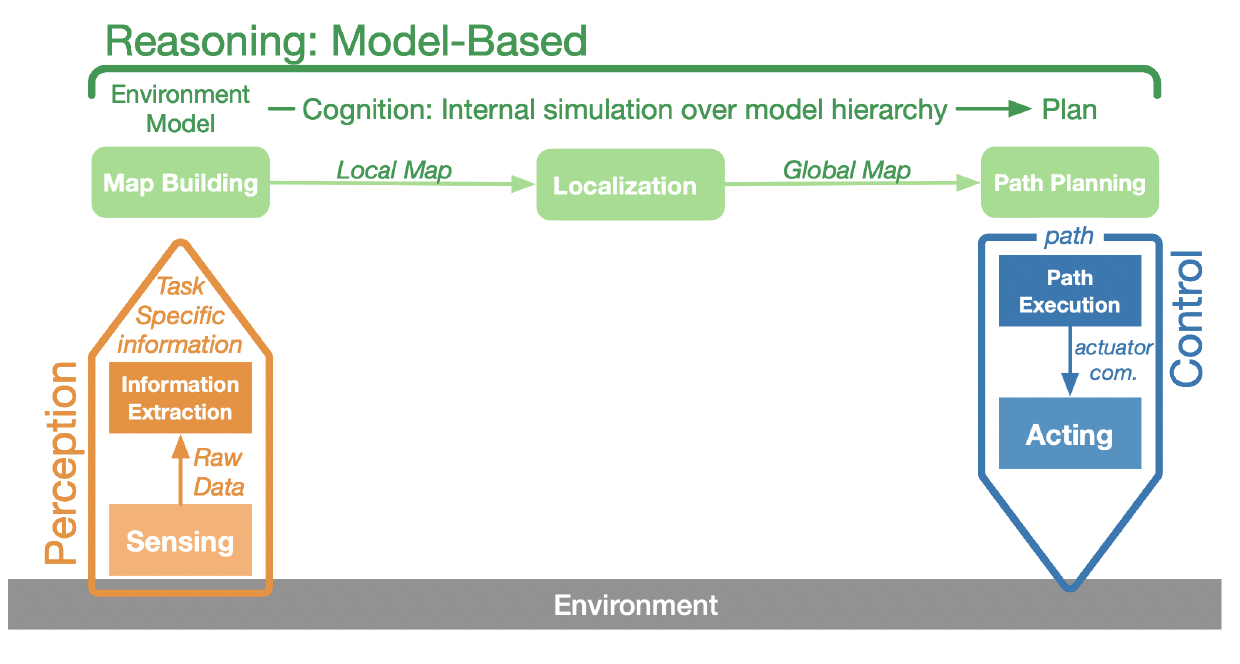
\includegraphics[width=0.7\textwidth]{Graphics/PRA}
		\caption{Perceive-Reason-Act \autocite{schillingAutonomeSystemeUnd2023}}
		\label{fig: fig1}
	\end{figure}
	
	
	\subsection{Development of Cognitive Architecture} 
	
	Cognitive Architecture is part of research in general AI and refers to the underlying frameworks that enable robots to mimic human-like cognitive processes. These architectures integrate perception, reasoning, and action to facilitate complex behaviors and decision-making in dynamic environments. By structuring robotic systems to process information, learn from interactions, and adapt to new situations, cognitive architectures aim to enhance the autonomy and intelligence of robots, enabling them to perform tasks that require high levels of understanding and adaptability.  \autocite{kotseruba40YearsCognitive2020} Given the dynamic and diverse nature of environments and applications, numerous definitions have been proposed for the key criteria that define a cognitive architecture. According to Newell \autocite{newellPrecisUnifiedTheories1992}, essential criteria for cognitive architectures include flexible behavior, real-time operation, learning, development, linguistic abilities, self-awareness, and brain realization. Sun \autocite{sunDesiderataCognitiveArchitectures2004} expanded this list to include broader concepts, such as ecological, cognitive, and bioevolutionary realism, modularity and synergistic interaction. However, differences in research goals, structure, operation, and application among existing cognitive architectures pose significant challenges for comparison and evaluation, making it near impossible to make a distinct defintion.  \autocite{kotseruba40YearsCognitive2020} Cognitive architectures, while powerful tools for modeling and understanding human cognition, come with several disadvantages. Despite their potential, the development and maintenance of cognitive architectures are complex and resource-intensive, demanding significant effort to build, debug, and extend. They often require substantial computational power and memory, which can limit their application in real-time scenarios or systems with constrained resources. Additionally, as these architectures grow in complexity, they can encounter performance bottlenecks, making scalability a challenge for larger, more intricate tasks. Integrating new modules or functionalities can also lead to integration issues and conflicts. \autocite{langleyCognitiveArchitecturesResearch2009, kotseruba40YearsCognitive2020} \newline
	
	%TODO: Komplett rauslöschen?
	Even though many of its advantages seem well-suited for our system, the drawbacks render cognitive architectures unsuitable for the purposes of this thesis, particularly in terms of adaptability, maintainability, and scalability. Consequently, we opted to explore alternative architectural types, with layered architectures emerging as the most viable option.
		
	\subsection{Layered Architectures}
	\textbf{Layered architectures} take a different approach to resolve the issues that the PRA model encountered. Horizontal layers of control systems are built to let the robot operate at increasing levels of competence and complexity and are assigned with different objectives. They consist of asynchronous modules which are allowed to communicate in a bidirectional manner. \autocite{brooksRobustLayeredControl1986} 
	Even though the higher levels can subsume the roles of lower levels by suppressing their output, the lower levels maintain their functionality as higher levels are added - resulting in a robust and flexible robot control system. \autocite{brooksRobustLayeredControl1986} An example of a layered architecture can be seen in Figure \ref{fig: fig2}, created by Brooks in 1986. \autocite{brooksRobustLayeredControl1986}
	

	\begin{figure}[ht]
		\centering
		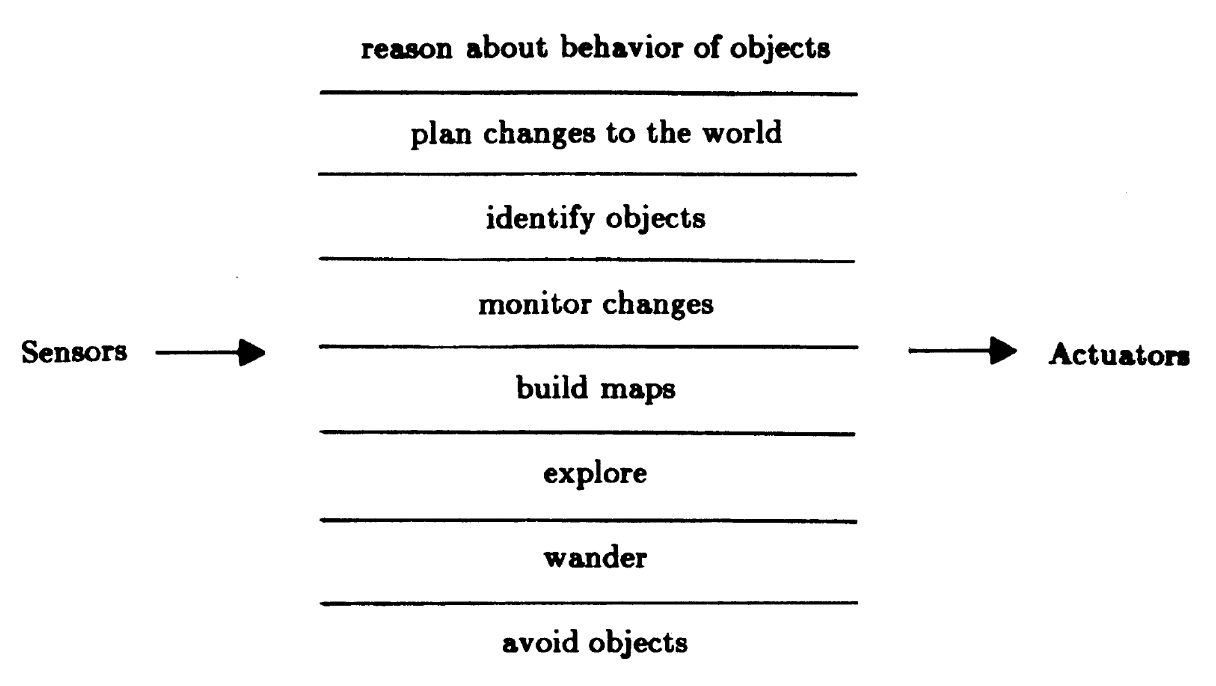
\includegraphics[width=0.7\textwidth]{Graphics/LayeredArchitecture}
		\caption{Layered architecture \autocite{brooksRobustLayeredControl1986}}
		\label{fig: fig2}
	\end{figure}
	
	Historically, layered architectures are composed of three layers: Behavioral layer, Executive layer and Planning layer. \autocite{jun-youngjungThreelayeredHybridArchitecture2008,peterbonassoExperiencesArchitectureIntelligent1997}
	
	\textit{The Behavioral layer} (also called the Hardware Abstraction-  or Functional layer) is typically found at the bottom of the hierarchy inside a layered architecture and provides a low-level library or interface to access the robot hardware, such as sensors or actuators. \autocite{jun-youngjungThreelayeredHybridArchitecture2008,simmonsLayeredArchitectureCoordination2002} It is often composed of very fast control loops, to create operations like path tracking or reflex-like reactions. \autocite{schillingAutonomeSystemeUnd2023} 
	
	\textit{The Planning layer} sits at the top of most architectures, making the decisions to achieve high level goals. This more complex and slower layer then sends the plans to the \textit{Executive layer}, which further decomposes tasks into subtasks. It is responsible for translating high-level plans into low-level behaviors, invoking behaviors at the correct times, monitoring execution, and handling exceptions. \autocite{schillingAutonomeSystemeUnd2023,simmonsLayeredArchitectureCoordination2002,volpeCLARAtyArchitectureRobotic2001} 
	As stated earlier, information and control is allowed to flow up and down through these layers, as the Behavioral layer sends back sensor data and actuator  information to the executive layer, which then informs the Planning layer on the current status of the assigned tasks. \autocite{jun-youngjungThreelayeredHybridArchitecture2008} A prototype of this structure can be seen in Figure \ref{fig: fig3}. 
	This architectural concept can even be extended to multiple robots, creating a sort of hive or swarm control, as Simmons et al. have shown in 2002. \autocite{simmonsLayeredArchitectureCoordination2002}
	
	\begin{figure}[ht]
		\centering
		\includegraphics[width=0.7\textwidth]{Graphics/three-layered-Architecture}
		\caption{Prototype three-tiered architecture \autocite{sicilianoSpringerHandbookRobotics2016}}
		\label{fig: fig3}
	\end{figure}
	\newpage
	
	\subsection{CLARATy}
	\label{subsec:CLARATY}
	While this typical three layered architecture is very popular and has been thoroughly investigated by developers, it does not come without its drawbacks. The developers of the "Coupled Layer Architecture for Robotic Autonomy" (\textbf{CLARATy}), a two layered architecture that is used for NASA's space robots \autocite{sicilianoSpringerHandbookRobotics2016}, identified three problems when designing three layered architectures:
	Firstly, the developers "expand the capabilities and dominance of the layer within which they are working" \autocite{volpeCLARAtyArchitectureRobotic2001}. This results in models, in which certain layers are predominantly active. Furthermore, there is still research to be done over the hierarchical superiority of the planning and executive layer of one over the other. \autocite{volpeCLARAtyArchitectureRobotic2001} Another problem the authors state is the lack of access from the Planning level to the Behavioral control. This forces the system to carry own models on the Planning layer, which are not directly derived from the functional layer, to perform planning tasks. Eventually, this can lead to inconsistencies between the layers and endanger the integrity of the system. \autocite{volpeCLARAtyArchitectureRobotic2001} Lastly, the authors claim that there is a misconception in equating greater intelligence in a system with increased granularity, suggesting that each part of a system can possess its own distinct hierarchy of granularity. They move on to explain that the Functional Layer contains many nested subsystems, the Executive layer encompasses multiple logic trees to coordinate these subsystems, and the Planning layer includes various timelines and planning horizons with different resolutions. \autocite{volpeCLARAtyArchitectureRobotic2001}
	In order to fight these challenges, Volpe et al. proposed a two layered architecture. This offers two main benefits: \newline
	Firstly, an explicit Representation of Granularity: CLARATy introduces a third dimension for granularity, allowing for a clearer depiction of the system's complexity and hierarchy. This means that within the Functional layer there's a detailed organization showing how subsystems are nested or grouped together. Secondly, they blended the Planning and Executive layer, resulting in a \textit{decision} layer which is more efficient and allowed the levels to share a common database (depicted in figure \ref{fig: fig4}). \autocite{volpeCLARAtyArchitectureRobotic2001} 
	
	
	\begin{figure}[ht]
		\centering
		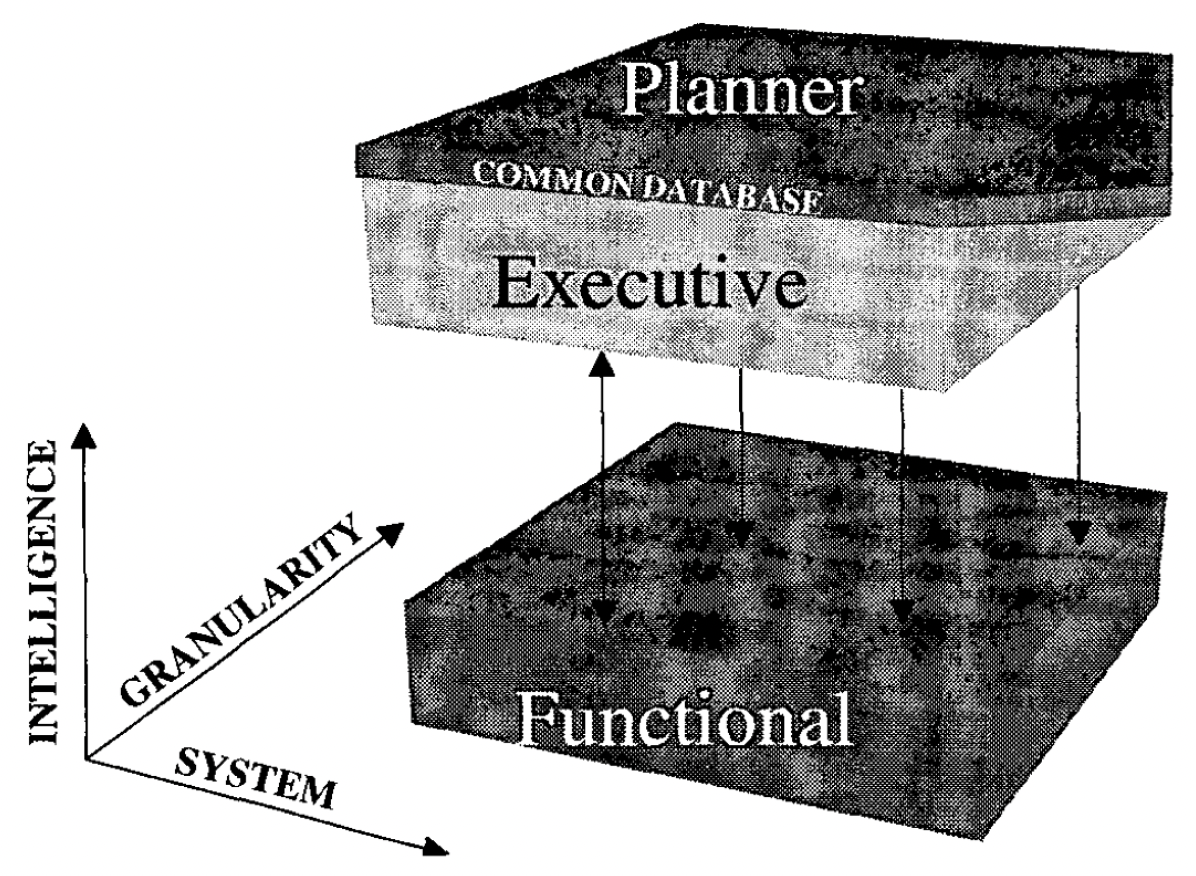
\includegraphics[width=0.7\textwidth]{Graphics/CLARATy}
		\caption{CLARATy architecture \autocite{volpeCLARAtyArchitectureRobotic2001} }
		\label{fig: fig4}
	\end{figure} 
	
	
	
	After this concise overview of some existing architectural systems, this thesis will now present the integral middleware that serves as the backbone of the proposed architecture.
	Understanding the principles of a layered architecture provides a solid foundation for appreciating the architectural choices and design patterns employed in robotic systems. As we have seen, there is no definitive way to construct these systems. Rather, this architecture type provides some key characterics by its division of system functionalities into distinct layers. Each layer fulfills a specific role and offers clarity, modularity, and scalability. As we transition our focus to the Robot Operating System (ROS), it becomes evident how ROS embodies these principles through its comprehensive framework for robot software development.
	
	
	
	\section{Robot Operating System}
	\subsection{ROS 1}
	The Robot Operating System (ROS) is an open-source operating system for robots. It provides the services expected from an operating system, including hardware abstraction, low-level device control, implementation of commonly-used functionality, message-passing between processes, and package management. ROS is not an operating system in the traditional sense of process management and scheduling. Rather, it is a framework or middleware upon which robotics software is developed, offering a structured communications layer above the host operating systems of a heterogeneous compute cluster. \autocite{quigleyROSOpensourceRobot2009,ros.orgIntroductionROS2024}
	ROS's architecture is designed around the notion of the intercommunication between numerous computing processes (often referred to as nodes) over a peer-to-peer network. This decentralized computing architecture enables the development and integration of complex robotic systems from modular and reusable components or packages. The system facilitates a distributed computing environment, allowing for the separation of tasks such as sensing, perception, decision-making, and actuation across multiple processors and machines. \autocite{quigleyROSOpensourceRobot2009}
	Central to ROS is its communications infrastructure, which enables the exchange of messages in various forms. These fundamental concepts include messages, topics, services and above mentioned nodes. The latter communicate with one another through messages ("strictly typed data structures" \autocite{quigleyROSOpensourceRobot2009}). This communication is implemented as a \textit{publisher-subscriber system:} On the one hand Nodes send messages to a topic by publishing the information, on the other hand nodes can receive the published information by subscribing to said topic. Multiple concurrent publishers and subscribers for the same topic may be active at any time. Also, a single node can publish and subscribe to many topics. \autocite{quigleyROSOpensourceRobot2009}
	Additionally, ROS provides capabilities for package management and a vast ecosystem of community-contributed tools and libraries that address various robotics functions ranging from planning and perception to simulation and visualization.
	\autocite{quigleyROSOpensourceRobot2009,ros.orgIntroductionROS2024}
	
	\subsection{ROS2 and its improvements}
	Even though ROS layed the groundwork for the modern robotic industry, the growing interest of industrial applications showed the limitations of ROS, which was built as a research platform. The urge for security, reliability in non-traditional environments and support for large scale embedded systems became the driver for the creation of ROS2, the second generation of the Robotic Operation System. \autocite{macenskiRobotOperatingSystem2022} 
	It introduces Node Lifecycle management, replaces the custom ROS1 middleware with industry standard middleware DDS (Data Distribution Service), better Real-Time support and adds Actions as a communicational tool. Actions in ROS2 are designed for long-duration tasks that require feedback to the caller during execution, which makes them distinct from the simpler service-call model.  \autocite{macenskiRobotOperatingSystem2022} A typical node interface for ROS2 can be seen in the figure \ref{fig: fig5} below. 
	
	\begin{figure}[ht]
		\centering
		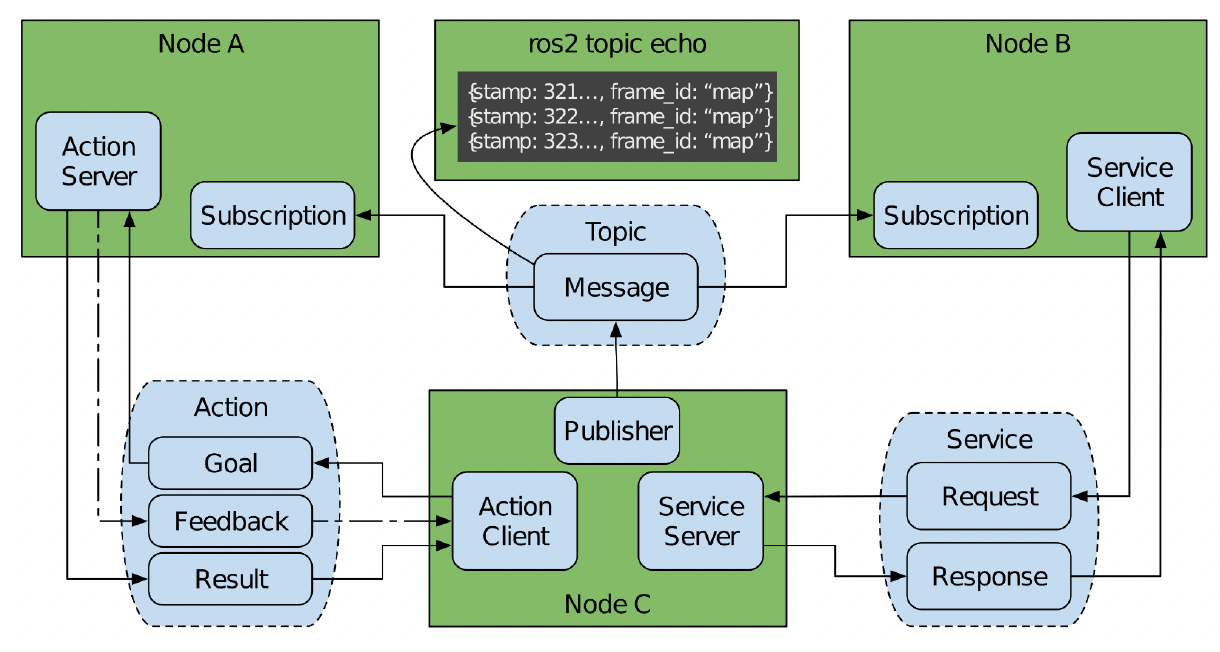
\includegraphics[width=0.7\textwidth]{Graphics/ROS2}
		\caption{ROS2 Node interfaces: topics, services and actions. \autocite{macenskiRobotOperatingSystem2022}}
		\label{fig: fig5}
	\end{figure}
	
	\section{How do you architect your robots?}
	\subsection{State of the Practice and Guidelines for ROS-based systems}
	Malavolta et al. \autocite{malavoltaHowYouArchitect2020} conducted a study in 2020 to answer three research questions: the architecture-relevant characteristics of ROS-based systems, the quality requirements considered in their design, and how to guide roboticists in architecting such systems. The authors used a two-part approach, mining ROS repositories and surveying developers who contributed to these repositories. The study found that ROS systems are becoming large and complex. While there are many open source packages and examples on how to use ROS, engineering robots with specific properties is still mostly an art of trial and error.The findings show that the most mentioned quality requirements related to ROS architecture were maintainability, performance, and reliability. The study also identified 39 guidelines for architecting ROS-based systems. These guidelines are useful for both roboticists aiming to develop high-quality robots and architecture researchers looking for evidence-based indications on how real-world ROS systems should be architected. I will now present 7 out of those 39 guidelines, which were evaluated as the most impactful for architectural design of robotic systems.
	\autocite{malavoltaHowYouArchitect2020}
	\subsection{Guidelines}
	\label{subsec:Guidelines}
	\begin{enumerate}[leftmargin=9mm, align=left]
		\item \textbf{Use standardized ROS message formats as much as possible, possibly supporting also their legacy versions.} 
		\item[]This first guideline emphasizes the importance of using standardized ROS message formats, particularly those from the common\_msgs and std\_msgs packages. Adopting these standards facilitates easier reuse, upgrade, and replacement of ROS nodes by allowing for straightforward topic remapping. Standardized messages enhance development efficiency by making compatible tools, such as visualizers and SLAM algorithms, easier available. They also improve node testability through isolation testing with ROS bags and simplify the integration of new sensors and hardware, as many manufacturers support ROS out of the box. However, since the definitions of standardized message formats are subject to change, it's crucial to design systems to be as decoupled as possible from specific message formats to ensure future compatibility and ease of updates. \autocite{malavoltaHowYouArchitect2020}
		
		\item \textbf{Group nodes and interfaces into cohesive sets, each with their own responsibilities and well-defined dependencies.} 
		\item[]Growing complexity poses a serious challenge while designing ROS-based software architectures, as it can result in hundreds of interdependent nodes leading to technical debt, limitations to certain ROS packages and reduce adaptability and extendability of the whole system. To mitigate these issues, the guideline suggests grouping nodes and interfaces into cohesive sets with defined responsibilities and dependencies. This structured approach aids in maintaining a clear understanding of the system's architecture, allowing for easier evolution and maintenance of the system. \autocite{malavoltaHowYouArchitect2020}
		\item \textbf{The behavior of each node should follow a well-defined lifecyle, which should be queryable and updatable at runtime.} 
		\item[]ROS inherits a certain flexibility that allows developers to create nodes without prescribed behaviors, offering great freedom but posing challenges for testability, reliability, and maintainability of stateful nodes. This guideline states the importance of treating node lifecycles as a crucial aspect of system design, suggesting documentation of node lifecycles to improve interaction, predictability, and test case development. As stated earlier, the development of ROS 2 already addresses some of these issues by supporting managed nodes with defined lifecycles (Unconfigured, Inactive, Active, Finalized) that can be inspected and controlled, enhancing testability and system management. Additionally, some ROS packages, even outside ROS 2's managed nodes, incorporate lifecycle considerations into their APIs, enabling runtime configurability and reflection to bolster system adaptability and autonomous capabilities. \autocite{malavoltaHowYouArchitect2020}  Defining and enforcing the lifecycle of ROS nodes "can enhance the system in terms of run-time configurability and reflection, which can be exploited for providing autonomous capabilities". \autocite{malavoltaHowYouArchitect2020}
		\item  \textbf{Assign meaningful names to components (e.g., nodes, topics, services) and group them by adopting standard prefixes/suffixes.} 
		\item[] This pretty self explanatory problem is especially importan in ROS-based systems, as topics and services are created programmatically by the nodes at run-time and their identifiers are simple strings. \autocite{malavoltaHowYouArchitect2020}
		\item  \textbf{Nodes directly interacting with simulators and hardware devices should provide identical ROS messaging interfaces to the rest of the system} 
		\item[] This guideline essentially boils down to creating uniformity in messaging interfaces, which allows developers to easily swap between simulations and hardware applications, while reducing modification cost to a minimum. \autocite{malavoltaHowYouArchitect2020}
		
		\item \textbf{ROS nodes should be resilient with respect to the amount and frequency of the data received by sensors.} 
		\item[] This principle highlights the challenges developers face when working with hardware sensors in robotics: Sensors often produce data in bursts, can degrade, and become less accurate over time. To handle these challenges, developers are advised to design their systems with flexibility in mind, by implementing load balancing nodes to manage sudden data surges and designing nodes to be resilient to gaps in sensor data. This resilience is crucial for the reliability of state estimation nodes, where faults can cause significant system-level failures. I expect this guideline to not be of great relevance in my project, due to the rather small(-ish) dataload. Nonetheless, a cruicial thought to keep in mind, when designind robotic systems. \autocite{malavoltaHowYouArchitect2020}
		
		\item \textbf{Avoid persisting raw data if only part of it will be used.}
		\item[] This guideline refers to the obstacle of how extensive data logging or storage operations can negatively impact the system's performance during its operation. Developers are advised to selectively record only the necessary data to avoid these performance issues. \autocite{malavoltaHowYouArchitect2020}
		
		
	\end{enumerate}
	
	The proposed architecture will try to adhere to these guidelines as much as possible, in order to create a robust and performant robotic system.
	
	
	\section{Niryo One Arm Architecture}
	The Niryo One is a collaborative and open-source 6-axis robot designed for research and higher education in the context of the industry 4.0.
	Its architecture has been mentioned by Malavolta et al. as an example, that adheres very well to above stated guidelines. \autocite{malavoltaHowYouArchitect2020} Niryo One operates upon a layered architecture, which is composed of five layers. Each layer is further subcategorized into different packages, among them pre-built ROS packages, imported libraries or self-created packages. \newline
	
	At the lowest level we can find the \textbf{Hardware layer}. This layer contains a package \textit{rpi} that handles all the external hardware (everything besides the motors) of Niryo One, and provides many utilities for the Raspberry Pi 3, such as Wi-FI, LEDs, Buttons etc. Furthermore, a \textit{driver} package is built, which provides an interface to ros\_control and handles the hardware control of motors. The other two packages found in figure \ref{fig: fig6} (\textit{dynamixel\_sdk} and \textit{mcp\_can\_rpi}) are imported libraries to stabilize functionality of the Raspberry pi and control the actuators. \autocite{roboticsNiryoOneROS2024} \newline
	
	Next up, a \textbf{control level} is implemented, which is entirely made up of the pre-built ros packages \textit{ros\_control} and \textit{joint trajectory controller}. The former is a set of packages that include controller interfaces, controller managers, transmissions and hardware interfaces \autocite{ros.orgROSControl2024a}, while the latter provides a controller for executing joint-space trajectories on a group of joints. \autocite{ros.orgJointTrajectoryController2024} \newline
	
	The actual motion control is invoked by the next higher level, the \textbf{Motion Planning layer}. Not only is there a \textit{description} package, containing the URDF file and meshes for Niryo One (which is essentially a description for the robot), but also the widely used \textit{moveit} packages, which is already part of the ROS ecosystem. The motion planning layer is responsible for finding inverse kinematics and building a path for the robot.\autocite{roboticsGetStartedNiryo2024,ros.orgMoveItConcepts2024} For each point, each axis are given a specific position, velocity, and acceleration. This path is sent to the joint trajectory controller for the actual hardware execution. \autocite{roboticsGetStartedNiryo2024}
	
	On top of that, the \textbf{Commander layer} provides a higher level interface between the client and the underlying robot commands. All commands, that the user inputs (e.g. "move joints"), go through this layer. The \textit{commander} package handles concurrent requests, validates parameters and calls required controllers and then returns appropriate messages and status. 
	Furthermore, a \textit{python\_api} package allows for easier access for other developers and tries to reduce the complexity of ROS for beginners. \autocite{roboticsGetStartedNiryo2024,roboticsNiryoOneROS2024}
	
	On the highest level, the architecture features a \textbf{External communication layer}.  This layer allows for communication outside the ROS ecosystem. First a TCP server is established in the \textit{modbus} package. It offers a simple way for developers to create programs for robot to control them via remote communication on a computer, on a mobile or any device with network capability. Lastly, the ROS-packages \textit{rosbridge} and \textit{joy} are imported, in order to allow communication between ROS1 and ROS2 and the use of the joystick controllers. \autocite{roboticsGetStartedNiryo2024,roboticsNiryoOneROS2024}
	
	
	\begin{figure}[ht]
		\centering
		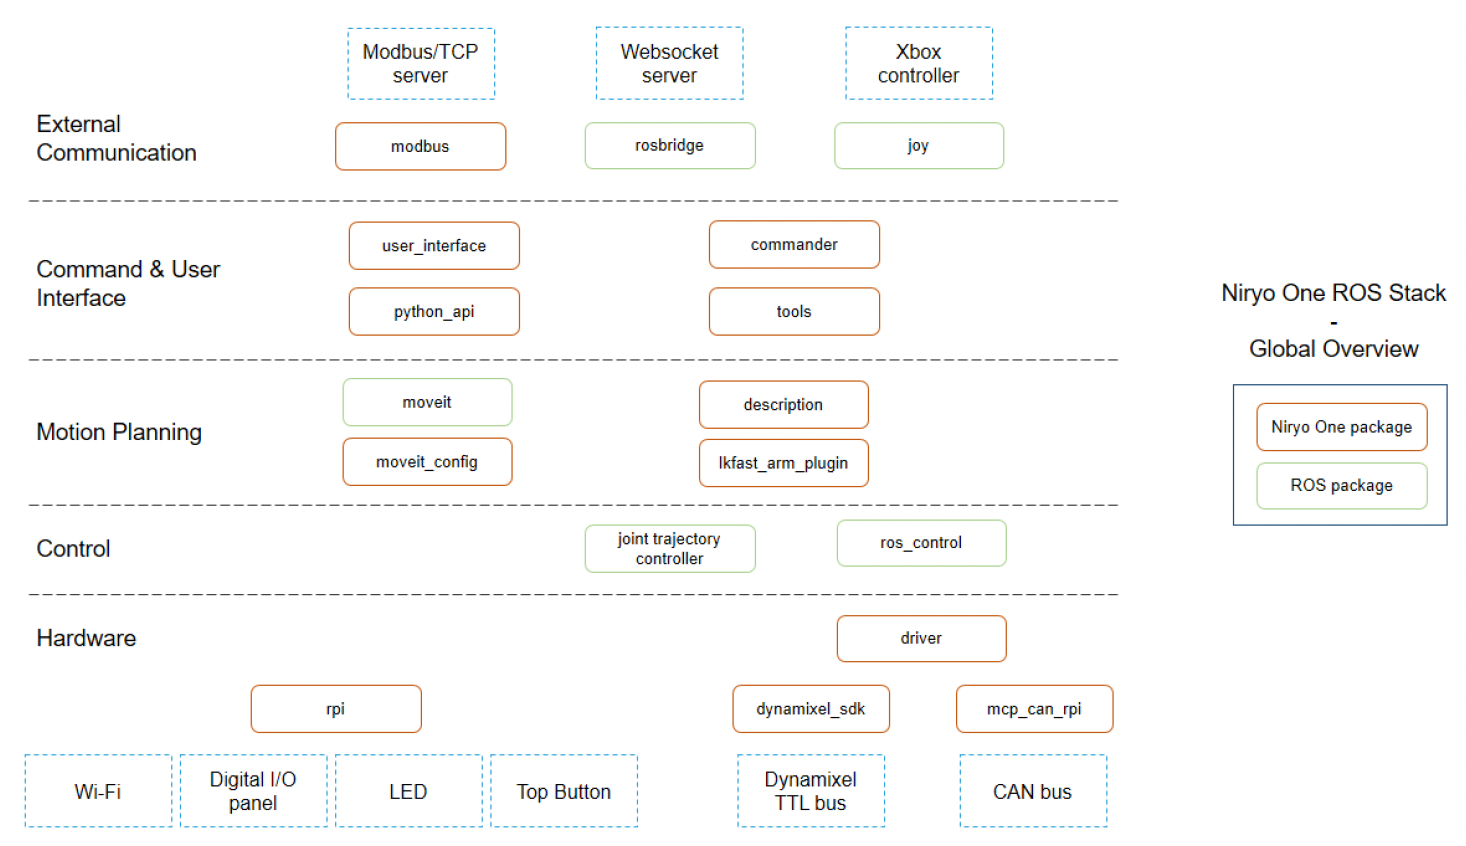
\includegraphics[width=0.9\textwidth]{Graphics/Niryo}
		\caption{Niryo One ROS Stack overview \autocite{roboticsNiryoOneROS2024}}
		\label{fig: fig6}
	\end{figure}
	
	After this thorough examination of existing architectures, we will now introduce our own approach to a layered robotic system. 
	
	
	\chapter{Methodology}
	\section{Frameworks and Setup}

	The architectural system is employed on the Turtlebot3 Burger Bot platform. This robot is frequently used in education and research because of its size, affordability and wide range of adaptability and expandability. A brief overview of the robots composition is shown in Figure \ref{fig: fig7}. 
		
	\begin{figure}[ht]
		\centering
		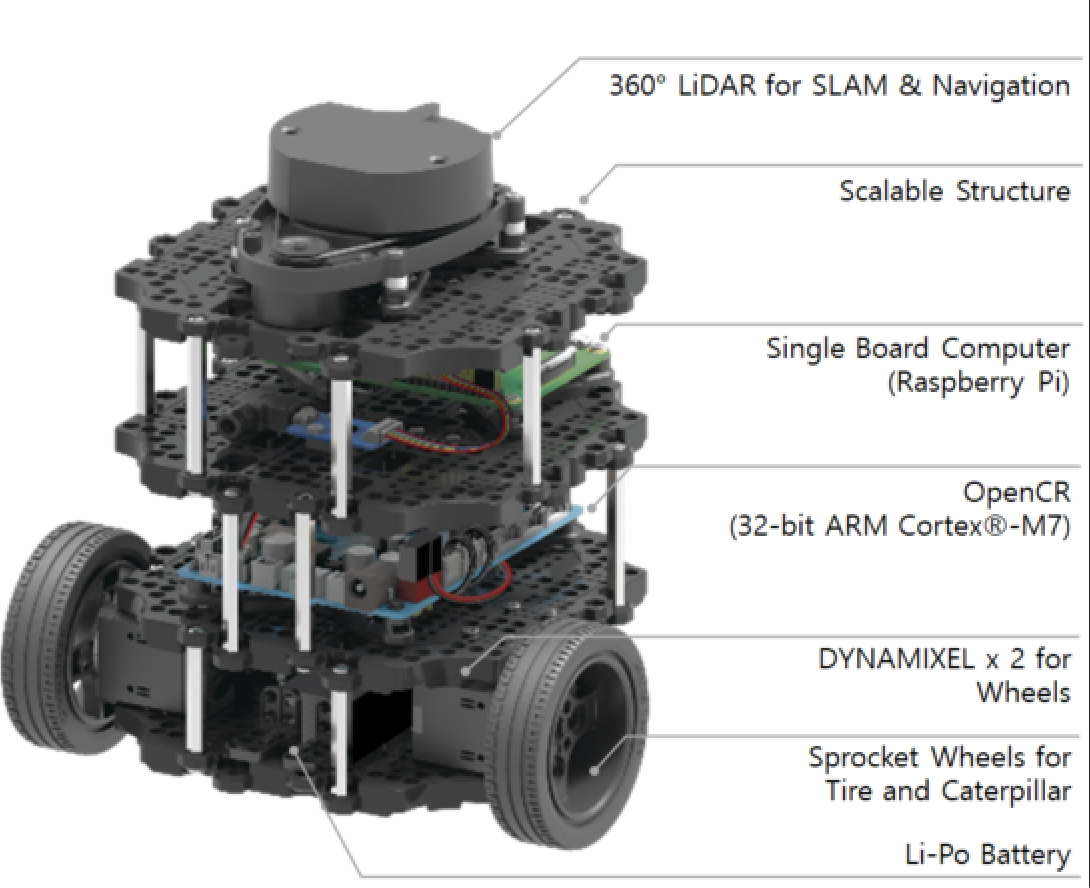
\includegraphics[width=0.5\textwidth]{Graphics/Turtlebot3}
		\caption{Turtlebot3}
		\label{fig: fig7}
	\end{figure}
		
	 The Architecture is built on the Ubuntu 22.04 LTS Operating System and ROS2 Humble for both the remote PC and the Raspberry Pi4 \footnote{ A Raspberry Pi is a small single-board-computer which is often used in robotics, because of its low cost, modularity and open design} on the Turtlebot3. The OpenCR board\footnote{ OpenCR is the Open-source Control Module for ROS. It is developed for ROS embedded systems to provide completely open-source hardware and software} is setup as instructed by the distributor of the Turtlebot3 platform ROBOTIS.\autocite{robotisEmanualROBOTIS2024} \newline
	 Any simulation is done with Gazebo Fortress (as required for ROS2 Humble) and RVIZ. 
	 Gazebo is a robust simulation environment used for testing and developing robotic algorithms in complex, realistic settings. It offers a precise physics engine, advanced 3D graphics, and supports a variety of sensors and actuators. RViz on the other hand is a 3D visualization tool for ROS that displays real-time data from sensors and robot models. It helps in debugging and analyzing robotic systems by providing insights into sensor perceptions and algorithmic decisions. RViz's customizable interface allows users to tailor visualizations to their specific needs, enhancing understanding and performance analysis of robotic systems. 
	 The different layers of the architecture are realised through Python and /Shell scripts, as well as some C/C++.  Each layer is essentially a ROS package, containing not only python scripts, but also setup.py or CMakeLists.txt files to configure system entry points and package.xml to resolve any dependency issues. A simplified version of the architectures directory tree can be seen in Figure \ref{fig:fig16} in the Appendix.
	 
	 In the next section, a detailed overview of the system is presented. 
	 
	 
	 
	\section{Architecture and Design}
	
	The architecture is structured into multiple distinct layers as shown in Figure \ref{fig: fig8}, which grow in complexity the higher the layer is placed in the diagram. Closely following the example set by the Niryo One architecture \ref{fig: fig6}, the overview distinguishes between pre-built ROS packages and custom-built components. Additionally, the control flow of the architecture is represented by arrows of different colors, each indicating a specific type of interaction. Green arrows signify a long-lasting invocation of a service, action, or publisher. Red arrows denote a one-time invocation of a new module using bash scripts. Grey arrows indicate suppression, while blue arrows represent access to a topic, service, action, or entire functions of another package.
			
	At the foundational level, the \textit{Hardware Control} package serves as the primary interface with the robot's physical components. It is the only layer [apart from the nav2 package, which we will get to later on] that processes and publishes commands directly to the robot's motors and sensors. This module's design includes a prioritization mechanism that manages conflicting commands to ensure that higher priority tasks, such as emergency stops, preempt other actions. The Hardware Control acts as a library of functions for the other layers to call upon, in order to create movement, e.g. "Drive Forward", "Turn Left", "Turn Right", "Turn by Angle" etc."). 
		
	Above that is the rather straightforward \textit{Obstacle Avoidance} layer, which continuously reads sensor output from the 'LaserScan' message \autocite{ros.orgLaserScanMessage2024a} and calls upon the hardware layer to immediately stop and rotate the robot. This command is sent with the highest possible priority. If the Obstacle Avoidance layer is missing or dysfunctional, a flag is set and the Hardware Control is prohibiting all movement commands, to ensure robot safety. 
	
	For map management, the architecture integrates a SLAM Toolbox. This tool is critical for building and updating the map while the robot navigates through its environment. The SLAM process simultaneously localizes the robot within the map and updates the map's structure based on new information gathered from the robot's sensors. This data is published through the /map topic, permitting access to other layers.
	
	In order to make use of the SLAM Toolbox and create a map, the robot has to wander around in its environment. This is realised through the \textit{Random Explore} layer, which does exactly what the name suggests: Randomly explore the surrounding area by invoking movement through the Hardware layer with lowest priority commands. 
	
	In the same package as the SLAM Node, a \textit{Map Change Detection} Module is located, which continuously monitors the environment for changes, updating the navigation map on a set frequency (currently 30 seconds). It uses a change detection algorithm that compares the current map state with new data collected by the robot, ultimately deciding when the map is robust enough to request the navigational layer to take over the robots movements. This request is executed via a bash script that launches a new terminal and invokes the desired navigational module.
	
	At the highest level, the \textit{Navigation Layer} provides autonomous navigation capabilities. It is important to note, that two concurrent navigational modules are placed inside this layer: One is custom built while the other employs the nav2 system, a commonly used navigational framework which provides a wide range of algorithms and functionalities to facilitate Path planning and directed movement. \autocite{macenskiMarathonNavigationSystem2020} Both modules dynamically calculate the most efficient paths to the designated targets, considering the current environmental layout and obstacles as previously mapped by the SLAM Toolbox. While the Nav2 package overrides any movement commands independently, the custom navigation module relies on the Obstacle Avoidance and Hardware Control packages to facilitate movement. Both navigational systems also suppress the Random Explore package by setting a flag and therefore preventing any callbacks inside the Random Explore layer. 
	
	Lastly, there are a couple more modules which provide analytical output for this thesis such as Maps, Heatmaps or position logging. These modules dont impact the robots behaviour in any case. Nonetheless, they are part of the architecture and are worth mentioning. Most importantly, a Heatmap Generator is placed in this \textit{Analysis layer}. As soon as any navigational functionality is invoked, it maps the robots position from the /odom frame to the /map frame and therefore creates a heatmap that matches the given dimensions by the SLAM Toolbox. Some examples of these heatmaps will be shown in Chapter 4.3.
	
			
	\begin{figure}[H]
		\begin{flushleft}
		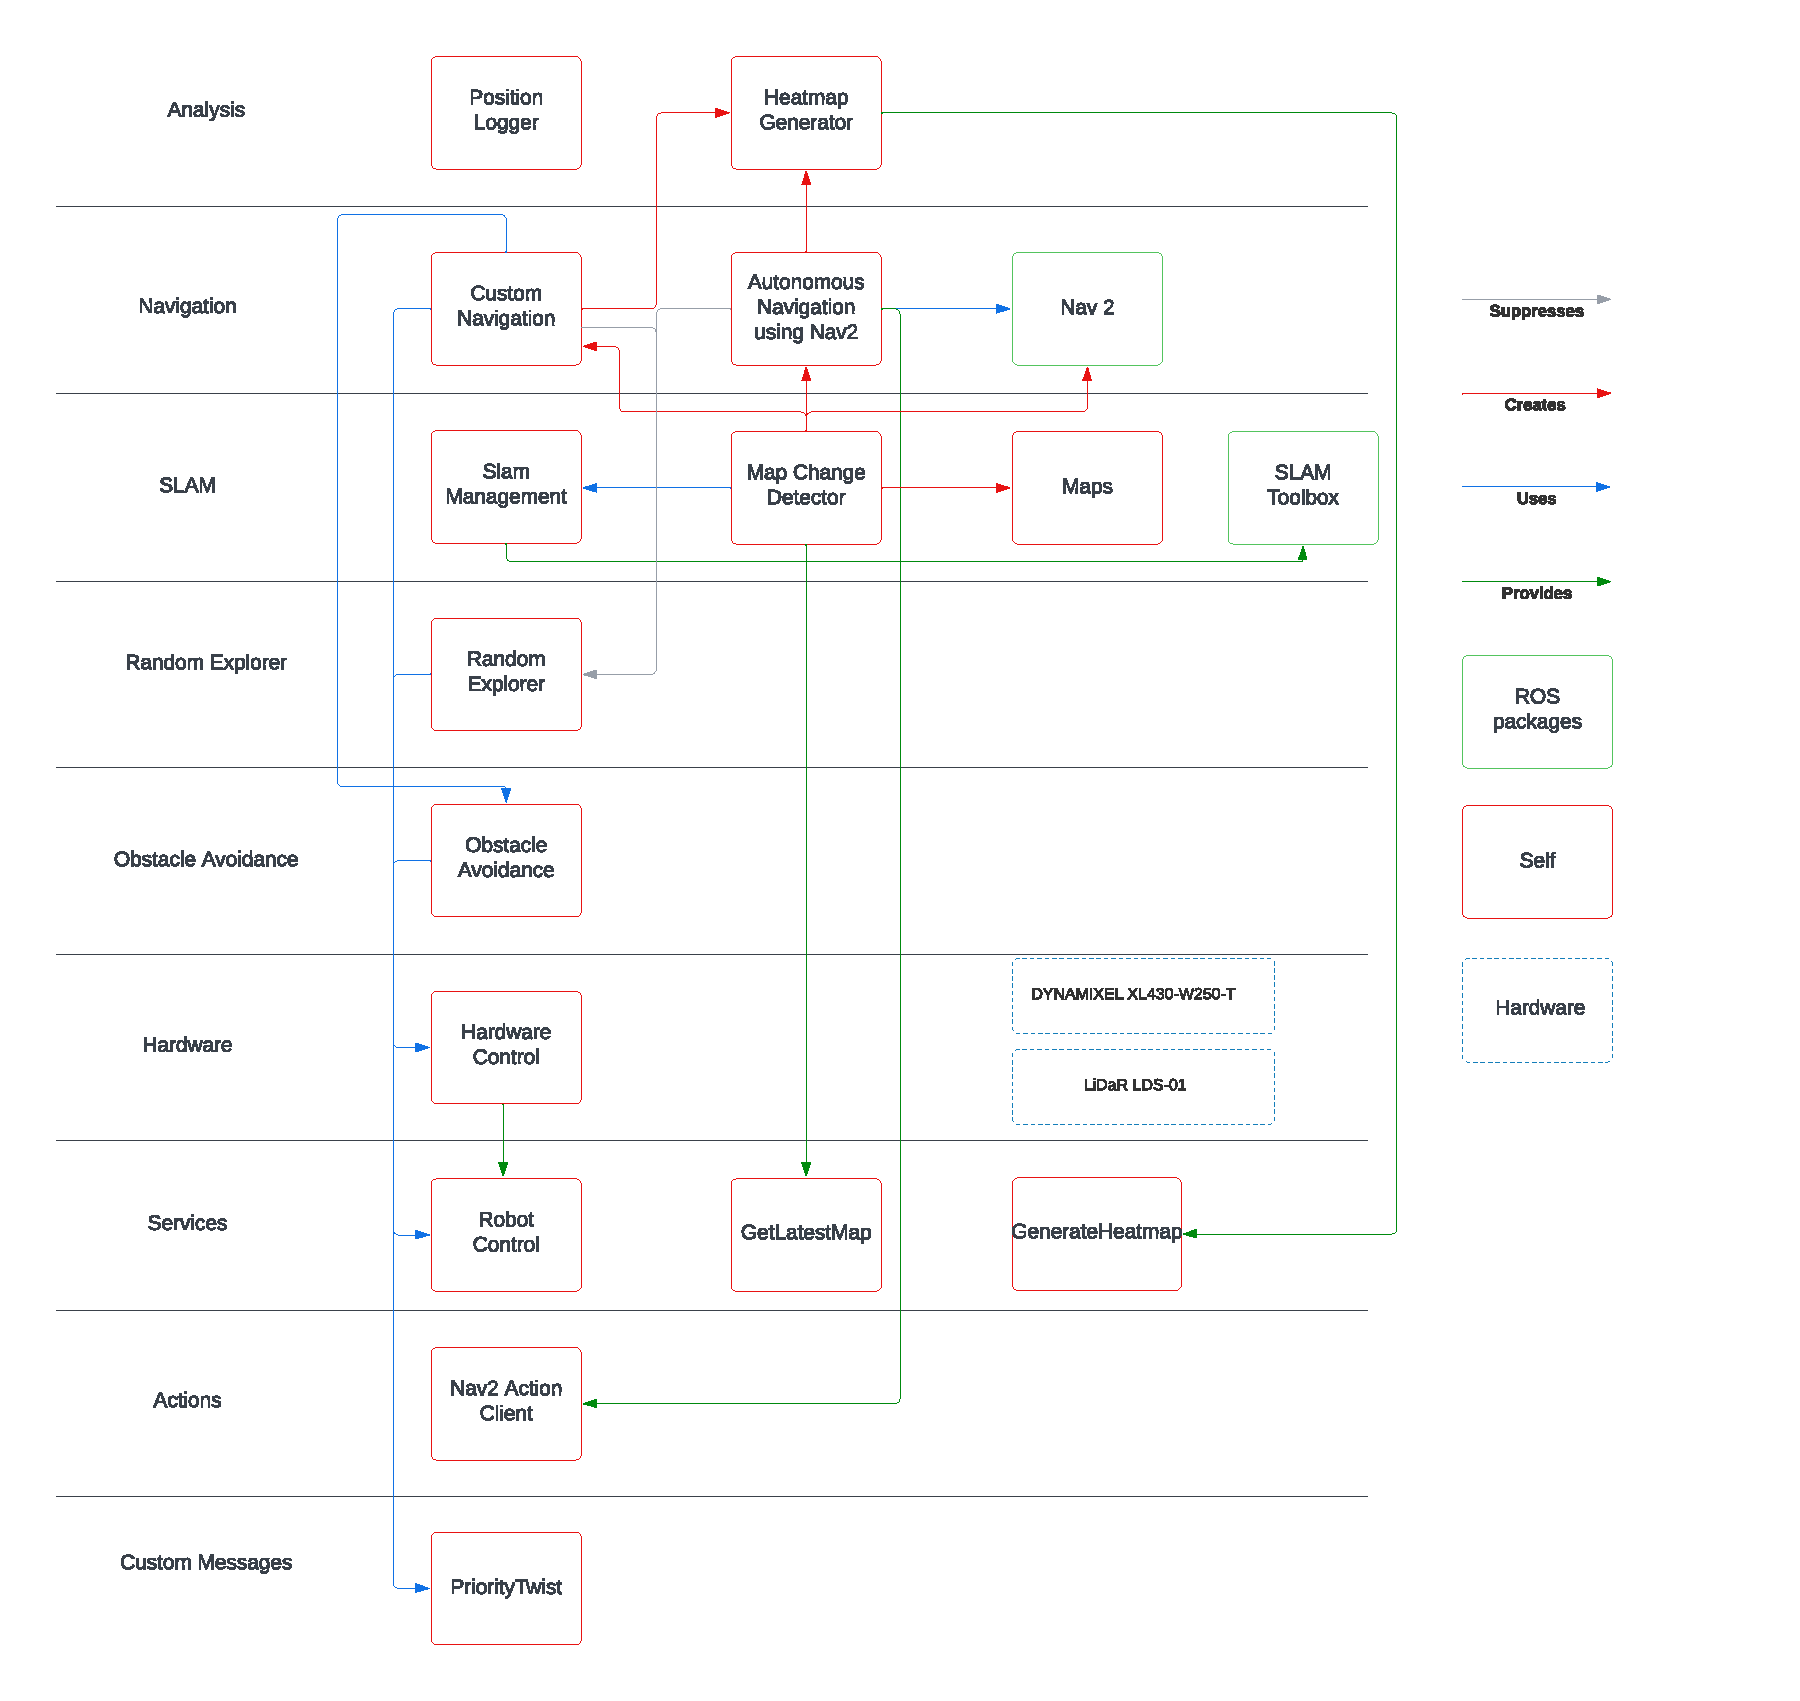
\includegraphics[width=1.3\textwidth]{Graphics/ArchitectureOverview}
		\caption{Architecture Overview. Boxes symbolize modules inside the layers. Arrows define control flow.}
		\label{fig: fig8}
		\end{flushleft}
	\end{figure}
	
	

	\chapter{Results}
	With the specifics of the architecture now established, we can analyze its adherence to the guidelines introduced by Malavolta et al. Subsequently, we move on to qualitative research in form of an ablation study.
	Since performing quantitative research on a layered architecture for robotic systems is relatively limited by the quantifiability of certain layers, this thesis then analyzes the performance of the two navigational systems. While their performance is undoubtedly significant, it is not the primary emphasis of this work. Instead, the thesis demonstrates the successful implementation of two interchangeable systems within the architecture, highlighting its modularity and adaptability. \newline
	 This analysis is mainly conducted in Gazebo and RViz, the prevalent simulation environments for robotic systems and ROS based applications. Following this, the application of the architecture on the real Turtlebot3 platform will be presented.
	\section{Comparison to Malavolta et al}
	\label{sec:ComparisonMalavolta}
	
	\begin{enumerate}[leftmargin=9mm, align=left]
		\item \textbf{Use standardized ROS message formats as much as possible, possibly supporting also their legacy versions.} 
		\item[]The architecture uses mostly standardized ROS message formats, such as LaserScan and Odometry. The external tools used in the system, such as SLAM Toolbox and Nav2, also use standardized ROS message formats: LaserScan, Odometry, Map and Twist. The only time the architecture deviates from this guideline is through the introduction of the custom PriorityTwist message. This design choice was made consciously, since the other possible solution for the prioritization mechanism involved environmental variables or global variables which not only are not common practice in Python, but also are very hard to maintain and reduce portability of the system. Furthermore, the priority is rather straightforward to understand, since it basically contains a normal Twist message at its core with only an added integer field.
		
		\item \textbf{Group nodes and interfaces into cohesive sets, each with their own responsibilities and well-defined dependencies.} 
		\item[]Since each layer provides a specific functionality in the greater system, dependencies are kept to a minimum and easily imported wherever needed. Apart from the standard ROS message dependencies, most layers only depend on the Hardware Control package (or rather the Robot Control service). An exeption makes the Navigational layer, which is connected to the vast framework of Nav2 and the SLAM Toolbox. These dependencies are necessary and therefore not within the inherent control of the architecture's design.
		
		\item \textbf{The behavior of each node should follow a well-defined lifecyle, which should be queryable and updatable at runtime.} 
		\item[]
		Each package in the system invokes and manages its own nodes, which is a result of the ROS2 Humble middleware with its managed nodes in order to enable runtime configurability. Furthermore, any node that is not initialized by the user at the start of robot operation has a well-defined lifecycle. Since the architecture is autonomous, most nodes are not designed to be updatable by user input at runtime, once their lifecycle has been invoked. 
		
		\item  \textbf{Assign meaningful names to components (e.g., nodes, topics, services) and group them by adopting standard prefixes/suffixes.} 
		\item[] The architecture establishes a standardized name convention. Any package is named ”turtlebot3 packagename”, with the corresponding node being named after the package name. Moreover, the entry points in the respective setup.py files follow the same name convention, resulting in rather straightforward terminal commands (e.g. ros2 run turtlebot3\_hardware\_control hardware\_control). 
		
		
		\item  \textbf{Nodes directly interacting with simulators and hardware devices should provide identical ROS messaging interfaces to the rest of the system} 
		\item[] When moving from simulator to hardware devices, the user only has to change a single flag in the bringup. Namely, the SLAM Toolbox expect a a boolean parameter ”use sim time”, which is set to true in simulation. This flag is queryable via the terminal, leaving the codebase untouched when transitioning environment.s Other than that, the system is indifferent to the usage of simulation or hardware application.
		
		\item \textbf{ROS nodes should be resilient with respect to the amount and frequency of the data received by sensors.} 
		\item[] As expected, the system encounters a rather small dataload from the lidar sensor. Furthermore, this dataload is comparably consistent. The absence of big sensor data has lead to little emphasis on this guideline. Therefore any addition to this system that increases sensor load needs to be tested thoroughly. Since the Obstacle Avoidance has its own managed node, faces a very small data load and operates on highest possible priority, the architectures robustness to system-level failure is suppsoedly quite high.
		
		\item \textbf{Avoid persisting raw data if only part of it will be used.}
		\item[] Apart from the map created by the SLAM Toolbox and any data generated for user visualization, no sensor data is persisted. However, there is no garbage collection system in place, which means that over many iterations of the model, a significant accumulation of maps and map configuration files may occur.
		
		
	\end{enumerate}
	
	\newpage
	
	
	\section{Ablation Study}  
	In order to further discuss the robustness of the architecture, an ablation study was conducted (see Figure \ref{fig: fig9}). The effect of an omitted layer on the other modules is categorized into three cases. Firstly, a layer can be completely unaffected, resulting in no changes to performance or robustness. Secondly, a layer can be indirectly affected by changes in other layers—meaning the layer itself does not directly access the contents or functionality provided by the omitted package but faces secondary consequences, such as an incomplete mapping of the environment. Thirdly, directly affected layers explicitly access the ommited layer and face severe repercussions in terms of unmet dependencies, unavailable services or other integral parts of the architecture. On the one hand, the omission of higher layers \footnote{\textit{Higher} and \textit{lower} layers are to be interpreted as shown in Figure \ref{fig: fig8}.} has no effect on the levels below it, which accounts for the lower triangular matrix of \textit{unaffected layers}. On the other hand, the removal of lower layers has varying impact on the levels above it. \newline 
	As expected, the ablation of the Hardware Control layer has a direct negative impact on all layers that rely on it to invoke movement, namely Obstacle Avoidance, Random Explore and the Custom Navigation. It also indirectly affects layers that rely on the robot being moved around (SLAM layer) and therefore by extension also the Navigation using Nav2, even though it overwrites any other movement commands and controls the robot on its own. \newline
	As a result of ommiting the Obstacle Avoidance module, the Random Explore layer cannot safely navigate the robot in an unknown environment, as the robot is very likely to crash into the first obstacle in its path. This culminates in an unfinished map, making any kind of navigation obsolete. The Custom Navigation also continuously accesses certain flags set in the Obstacle Avoidance package and is therefore directly affected. \newline
	The ablation of the Random Explore layer inherits the same problems we just described, with the exception that the Custom Navigation is not directly accessing said layer. \newline
	Clearly, the exclusion of the SLAM and Map Change Detector layer results in both navigational systems failing on multiple levels: Not only is no data being published to the /map topic, that both navigation systems heavily rely on, but both packages are also never invoked in the first place.  
	Lastly, it is evident that the two navigational packages do not interfere with one another and can functionally coexist - provided a given priority between the two navigational system is established. This means they are practically interchangeable and therefore qualify as a unaffected layer. 
	Note that the ablation of either navigational package during runtime does not interfere with the robot's ability to navigate safely in both simulation and real-world environments. Since a flag is set during the runtime of the navigation packages to suppress the Random Explore layer, the removal of the navigational module leads to a fallback to random exploration. Also, if the Obstacle Avoidance layer is missing, a similar flag is set to prohibit movement commands issued by the Hardware Control layer, ensuring that robot safety is prioritized above all else.
	
	
	\begin{figure}[H]
		\centering
		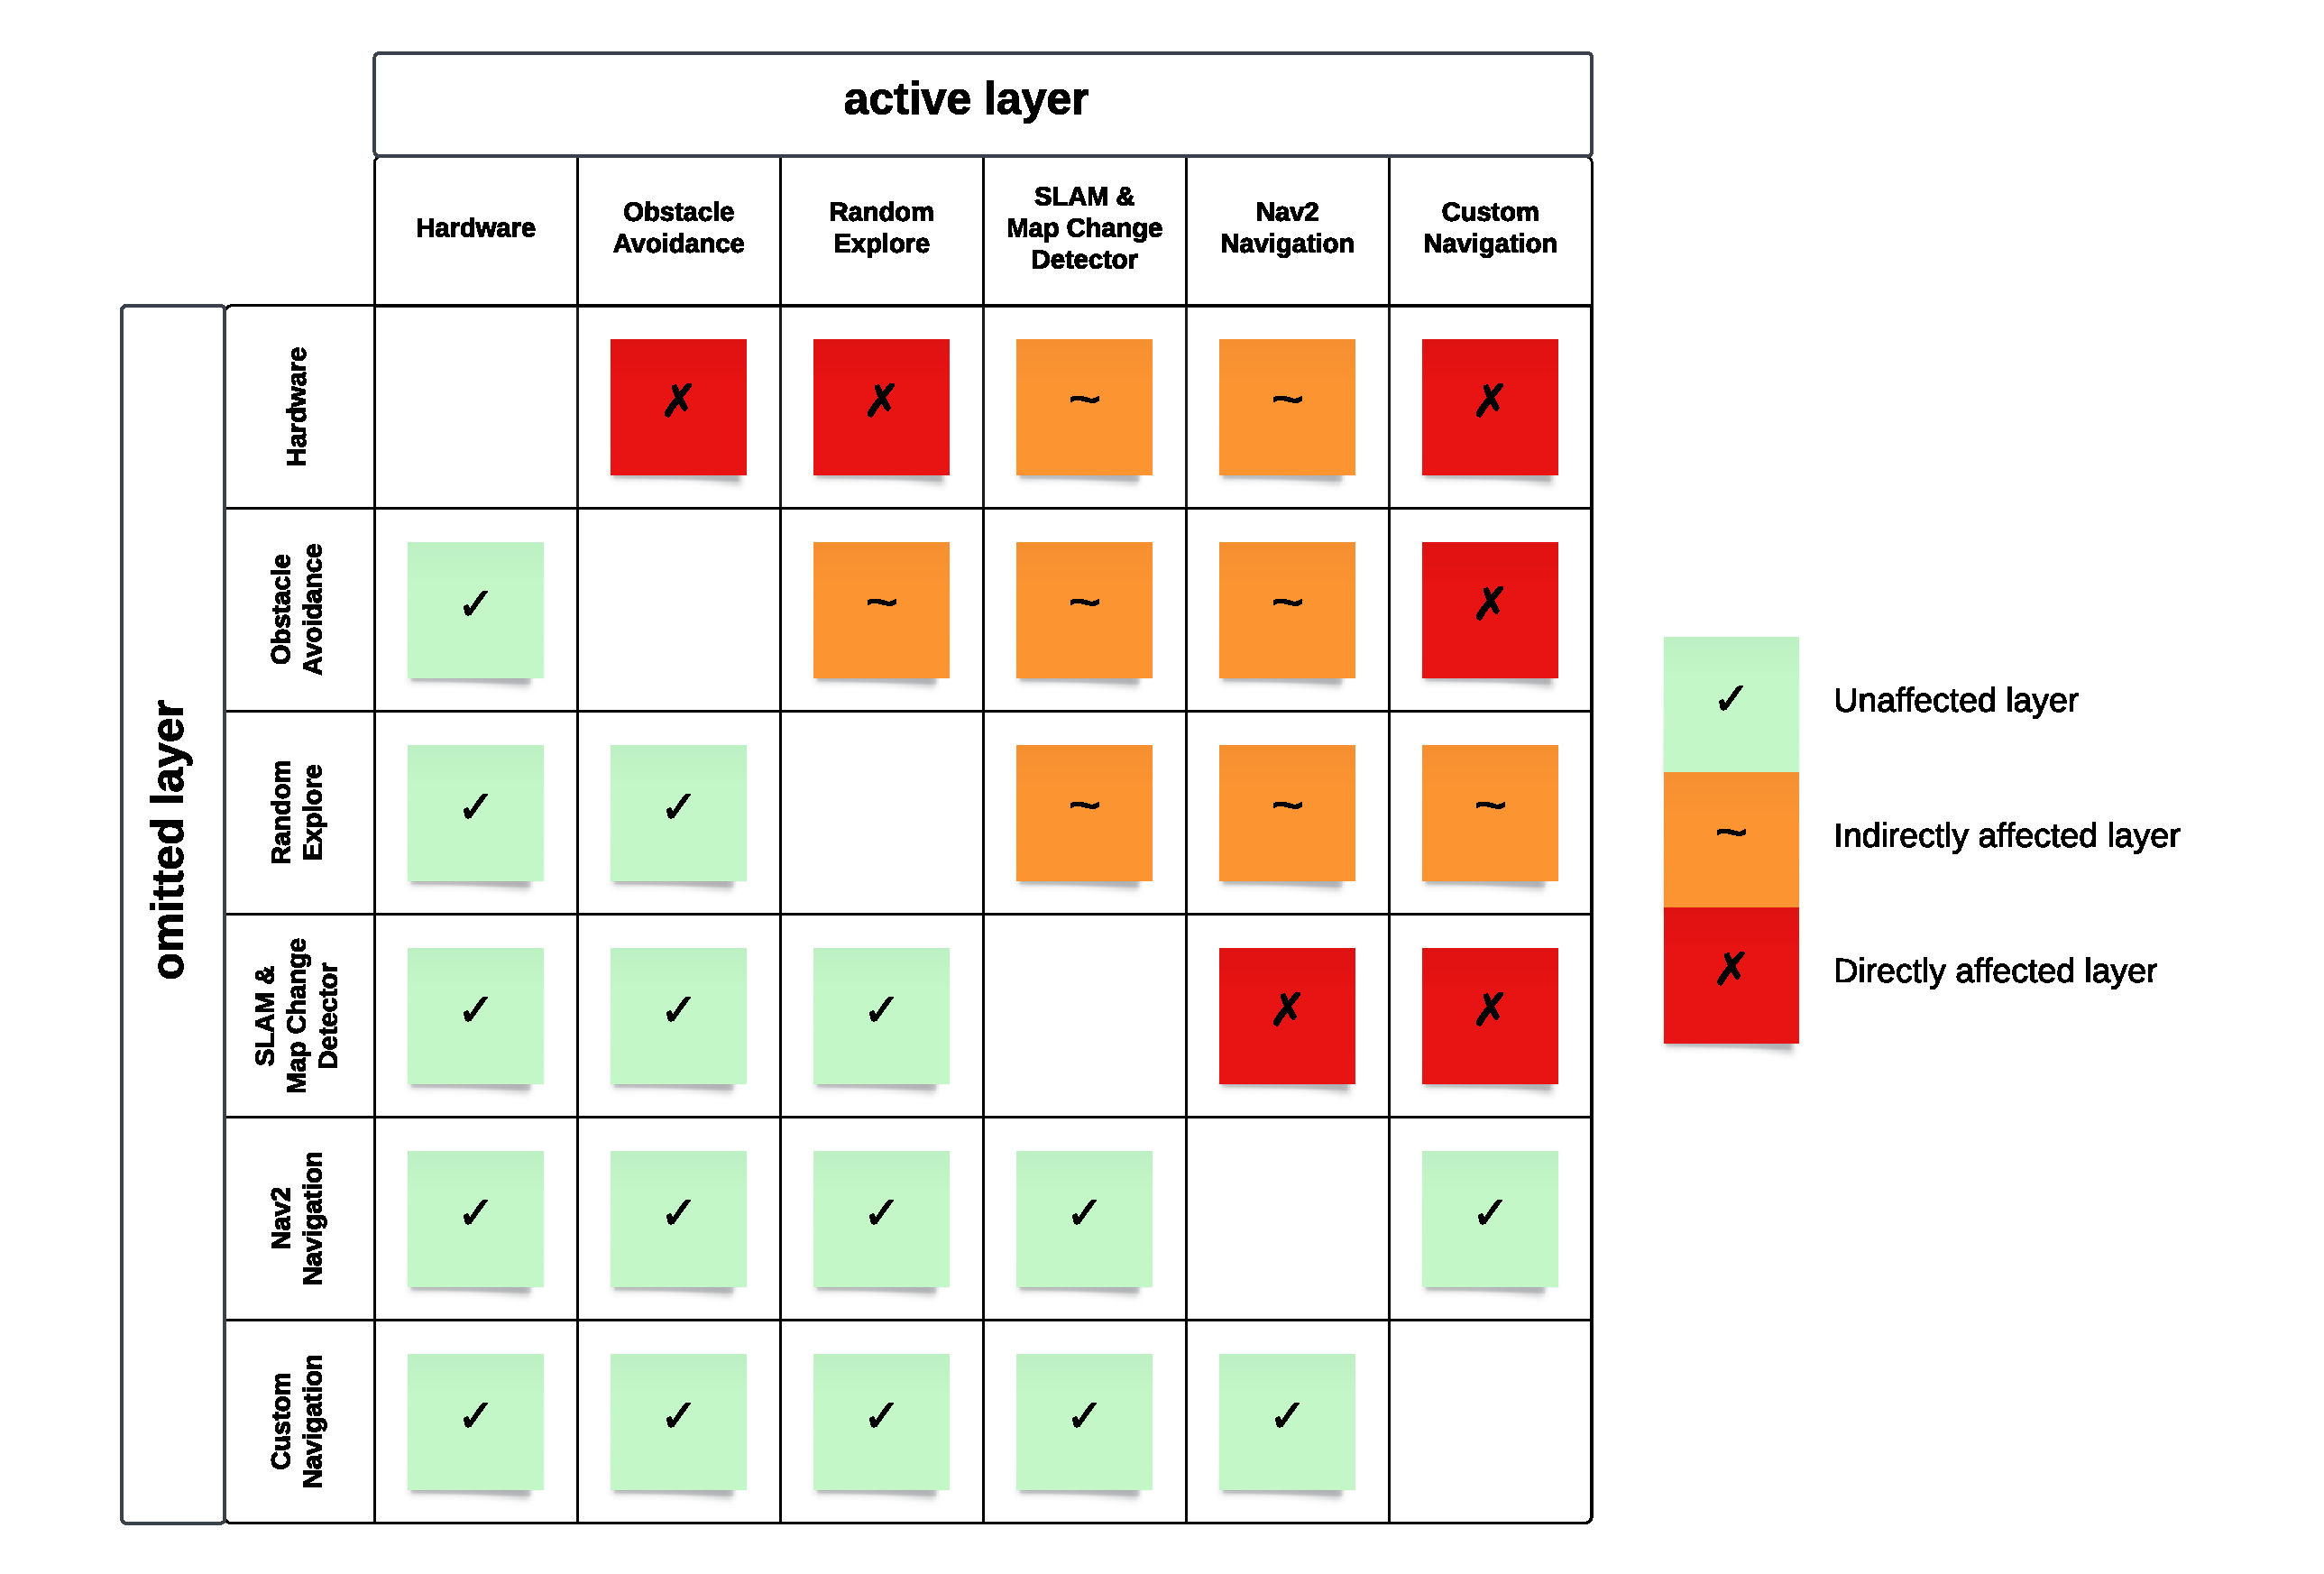
\includegraphics[width=0.9\textwidth]{Graphics/AblationStudy}
		\caption{Ablation Study on layer functionality}
		\label{fig: fig9}
	\end{figure}
	
	It becomes evident that the lower levels are vital for the performance and robustness of the architecture, while higher layers are more likely to have less devastating effects on overall stability or simply enhance the system's functionality. This additive nature results in a more adaptive and flexible design, as higher-level modules can easily be replaced by others with similar purposes. In contrast while examining the upper triangular matrix of figure \ref{fig: fig9}, it is inevitable to mention the dependency of the higher levels on the lower layers. This interdependence limits the overall flexibility of the architecture by how resilient and adaptable the lower layers are designed. 
	
	After this thorough analysis of the architectures resilience and robustness, we now move on to assess the systems performance. This evaluation will be divided into a simulated environment and an application to a real surrounding. 
	\section{Simulation} 
	The robot was provided with four distinct coordinate sets to navigate between. Each tuple of coordinates was targeted 20 times. While moving, two key metrics were collected: Distance traveled and the time used to get there. The full datasets for each iteration can be seen in the Appendix. Note that all coordinates were chosen at random and do not contain any bias towards one another, but both navigation systems where given the same coordinates. 
	To condense the findings, the mean and variance of the two metrics are calculated and shown in their respective tables. Furthermore, the movement of the robot was monitored via a heatmap, that was then projected onto the map provided by the SLAM Toolbox and Map Change Detection module.
	
	\subsection{Navigation using Nav2}
	Deploying the architecture with the Navigation based on the Nav2 package shows very coherent data. The Robot has used the same route through every iteration of the simulation, with the exception of one run in Coordinate Set 1 (see Figure \ref{fig:heatmaps} (a)). Near the destinations, the paths show some slight variance, which is attributed to the robots orientation when aligining its position to the correct coordinates. 
	
		\begin{figure}[H]
		\centering
		\begin{subfigure}[b]{0.45\textwidth}
			\centering
			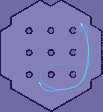
\includegraphics[width=\textwidth]{Graphics/heatmapsim1.png}
			\caption{Coordinate Set 1}
			\label{fig:fig10}
		\end{subfigure}
		\hfill
		\begin{subfigure}[b]{0.45\textwidth}
			\centering
			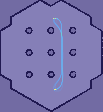
\includegraphics[width=\textwidth]{Graphics/heatmapsim2.png}
			\caption{Coordinate Set 2}
			\label{fig:fig11}
		\end{subfigure}
		\vfill
		\begin{subfigure}[b]{0.45\textwidth}
			\centering
			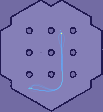
\includegraphics[width=\textwidth]{Graphics/heatmapsim3.png}
			\caption{Coordinate Set 3}
			\label{fig:fig12}
		\end{subfigure}
		\hfill
		\begin{subfigure}[b]{0.45\textwidth}
			\centering
			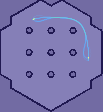
\includegraphics[width=\textwidth]{Graphics/heatmapsim4.png}
			\caption{Coordinate Set 4}
			\label{fig:fig13}
		\end{subfigure}
		\caption{Heatmaps using Nav2 package for all Coordinate Sets (n=20)}
		\label{fig:heatmaps}
	\end{figure}
	
	Another factor contributing to this frayed path is the robot's need to turn at the beginning of every iteration. The direction in which the robot turns is seemingly random and varies heavily in time used and turning radius. That is also why table \ref{tab:1} shows little variance in distance traveled, but quite a lot of variance in time used. \newline 
	Nevertheless, the long established and [compared to the Custom Navigation] rather sophisticated Nav2 package provides great performance for navigation on the Turtlebot3 platform.  

	
	
	\begin{table}[H]
		\centering
		\begin{tabular}{|c|p{3cm}|p{3cm}|p{3cm}|p{3cm}|}
			\hline
			Coordinate Set & Mean Distance \newline Traveled (m) & Variance Distance \newline Traveled (m) & Mean Time \newline Used (s) & Variance Time \newline Used (s) \\
			\hline
			0 & 5.306683 & 0.148930 & 27.932736 & 2.545896 \\
			1 & 4.065978 & 0.222748 & 21.998405 & 1.444408 \\
			2 & 4.395432 & 0.149748 & 22.895346 & 1.698574 \\
			3 & 4.173309 & 0.148584 & 22.000601 & 1.441569 \\
			\hline
		\end{tabular}
		\caption{Summary Statistic for Navigation using Nav2 package (n=20)}
		\label{tab:1}
	\end{table}
	
	
	\subsection{Custom Navigation}
	tbd
	%TODO
	
	\section{Real World Application} 
	{\color{red} Subject to change, falls ich das Problem noch lösen kann :( }
	Applying the layered architecture to a real environment is certainly the most difficult task during the creation of this thesis. While simulations provide a controlled and repeatable setting for initial development and testing, they cannot fully capture the complexities and unpredictability of a real environment. As seen in Figure \ref{fig:fig14}, the robot was placed in a square room with a couple of obstacles to avoid. The lower layers, namely Hardware Control, Obstacle Avoidance, Random Explore, SLAM Toolbox and Map Change Detector, worked as expected, resulting in the creation of the map as seen in Figure \ref{fig:fig15}. However, transitioning all layers from simulation to a real-world scenario presented significant difficulties. Although the SLAM Toolbox provides a .yaml file containing the essential details for mapping the robot's position (published by the /odom topic) to the frame of the /map topic, the navigational systems were either dysfunctional or imprecise, depending on the iteration. The efforts to debug these issues were severely constrained by the extensive time required for setting up the entire system, which includes charging, map creation, and actual navigation attempts.
	
			
	\begin{figure}[H]
		\centering
		\begin{subfigure}[b]{0.45\textwidth}
			\centering
			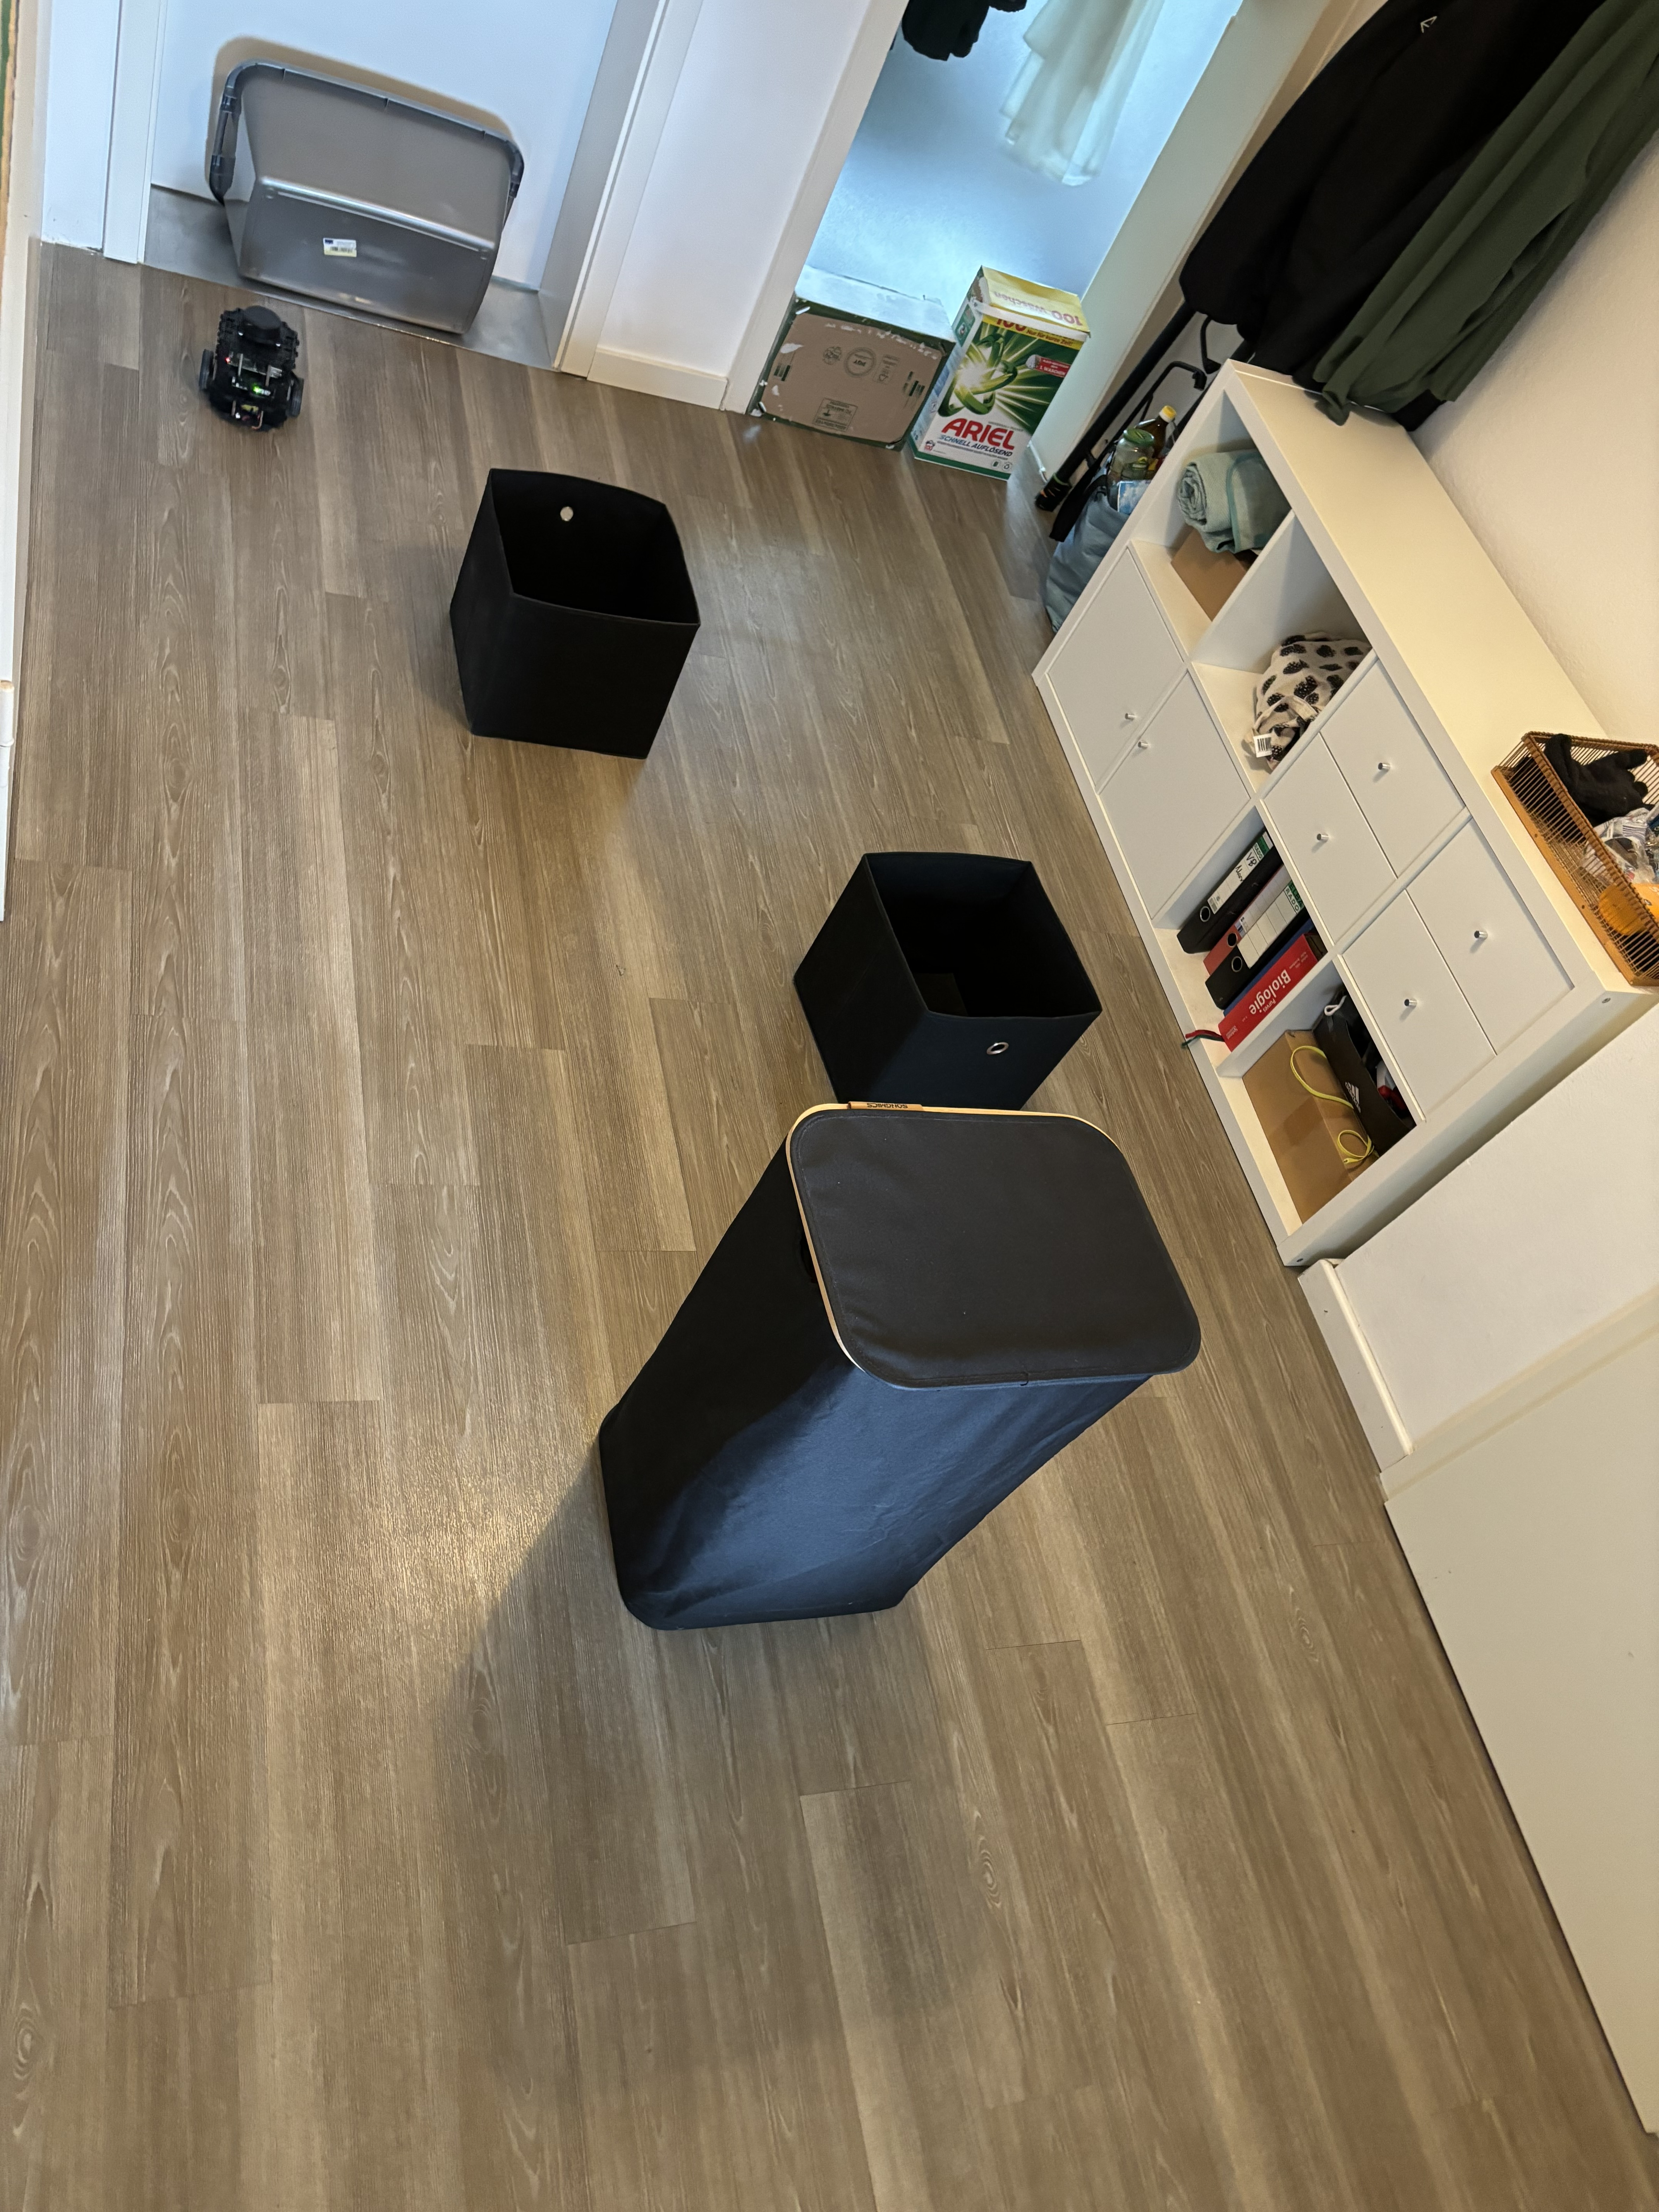
\includegraphics[width=\textwidth]{Graphics/RealWorldSetup.jpeg}
			\caption{Real World Setup (JPEG)}
			\label{fig:fig14}
		\end{subfigure}
		\hfill
		\begin{subfigure}[b]{0.45\textwidth}
			\centering
			\rotatebox{180}{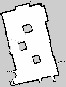
\includegraphics[width=\textwidth]{Graphics/RealWorldSetup.png}}
			\caption{Map by Turtlebot3}
			\label{fig:fig15}
		\end{subfigure}
		
		\caption{Real Environment and corresponding Map created by Turtlebot3}
		\label{fig:RealWorldSetup}
	\end{figure}	
	
	
	\chapter{Discussion}
	The primary aim of this thesis is to develop a layered architecture that is not only performant and robust but also modular, easily adaptable and maintainable. Supposedly, the system is designed to be horizontally structured with minimal vertical dependencies to enhance modularity and facilitate a plug-and-play environment. \newline
	
	In order to evaluate the architecture, the first step is to examine the conformity to the proposed guidelines by Malavolta et al. (see \ref{subsec:Guidelines} and \ref{sec:ComparisonMalavolta}). 
	Overall, the architecture adheres well to said principles: The majority of message formats used are standardized ROS messages, with only one exception: the custom Priority Twist message. The nodes follow a well-defined lifecycle and clear naming conventions, are agnostic to the use of simulators or hardware devices, and are logically grouped within their packages. It is important to note that Guideline 6 fell a little bit out of scope. Due to the relatively small amount of data and the infrequency of sensor data outages, the primary focus was directed towards other aspects. Consequently, no fallback plans, aside from retrying or waiting for the next data load, were implemented.
	Above statements are partially supported by the results of the ablation study and quantitative analysis. On the one hand, the ablation study \ref{fig: fig9} demonstrates that the system is robust when scaling upwards, indicating that adding new layers is safe and does not compromise the overall stability or performance of the architecture. On the other hand, the ablation study illustrates that creating a complex layered architecture is not feasible without vertical dependencies. These vertical dependencies become especially prevalent the lower the layer is set in the architecture, as these layers provide the most basic and essential functionalities such as movement and obstacle avoidance. A possible solution would be to overwrite those lower levels, as exemplified by the nav2 package. However, this bypass would not come without consequences, as complexity and responsibility in the higher levels would drastically increase, defeating the purpose of this architecture type. This expansion of capabilities and dominance of certain layers is also what the authors of the CLARATy architecture deemed the most problematic in past attempts to build robust architectures. \newline
	
	The employment of two concurrent navigational modules underlines the architecture's modularity and adaptability, as there is no upward dependency from a lower level to the navigational layer. This means that any navigational system can be implemented, provided it either adapts to the Hardware Control to invoke movement or suppresses the Hardware Control and invokes movement itself. \newline 
	
	The real-world application of the architectural system also provides two critical insights: While no layer required codebase adaptation to transition from simulation to hardware, only the lower layers were able to provide their designated functionality. However, this limitation could very well be attributed to my inability to create a functioning and robust navigational system and is not inherently a flaw in the architecture's design. {\color{red} @Malte: schreibt man so etwas? und wenn ja, wie?} \newline 
	This poor performance on the actual robot may also be ascribed to the lack of focus on guideline six, as data frequency received by the sensors might vary from simulation to real-world applications.
	
	TODO: Vergleich Nav2 und custom nav und deren performance/robustness
	
	%TODO: Vergleich Nav2 und custom nav
	

	\chapter{Conclusion}
	
	
	%TODO: 
	
	
	\printbibliography
	
	\chapter*{Appendix}
	\addcontentsline{toc}{chapter}{Appendix}
		
	\begin{figure}[H]
		\centering
		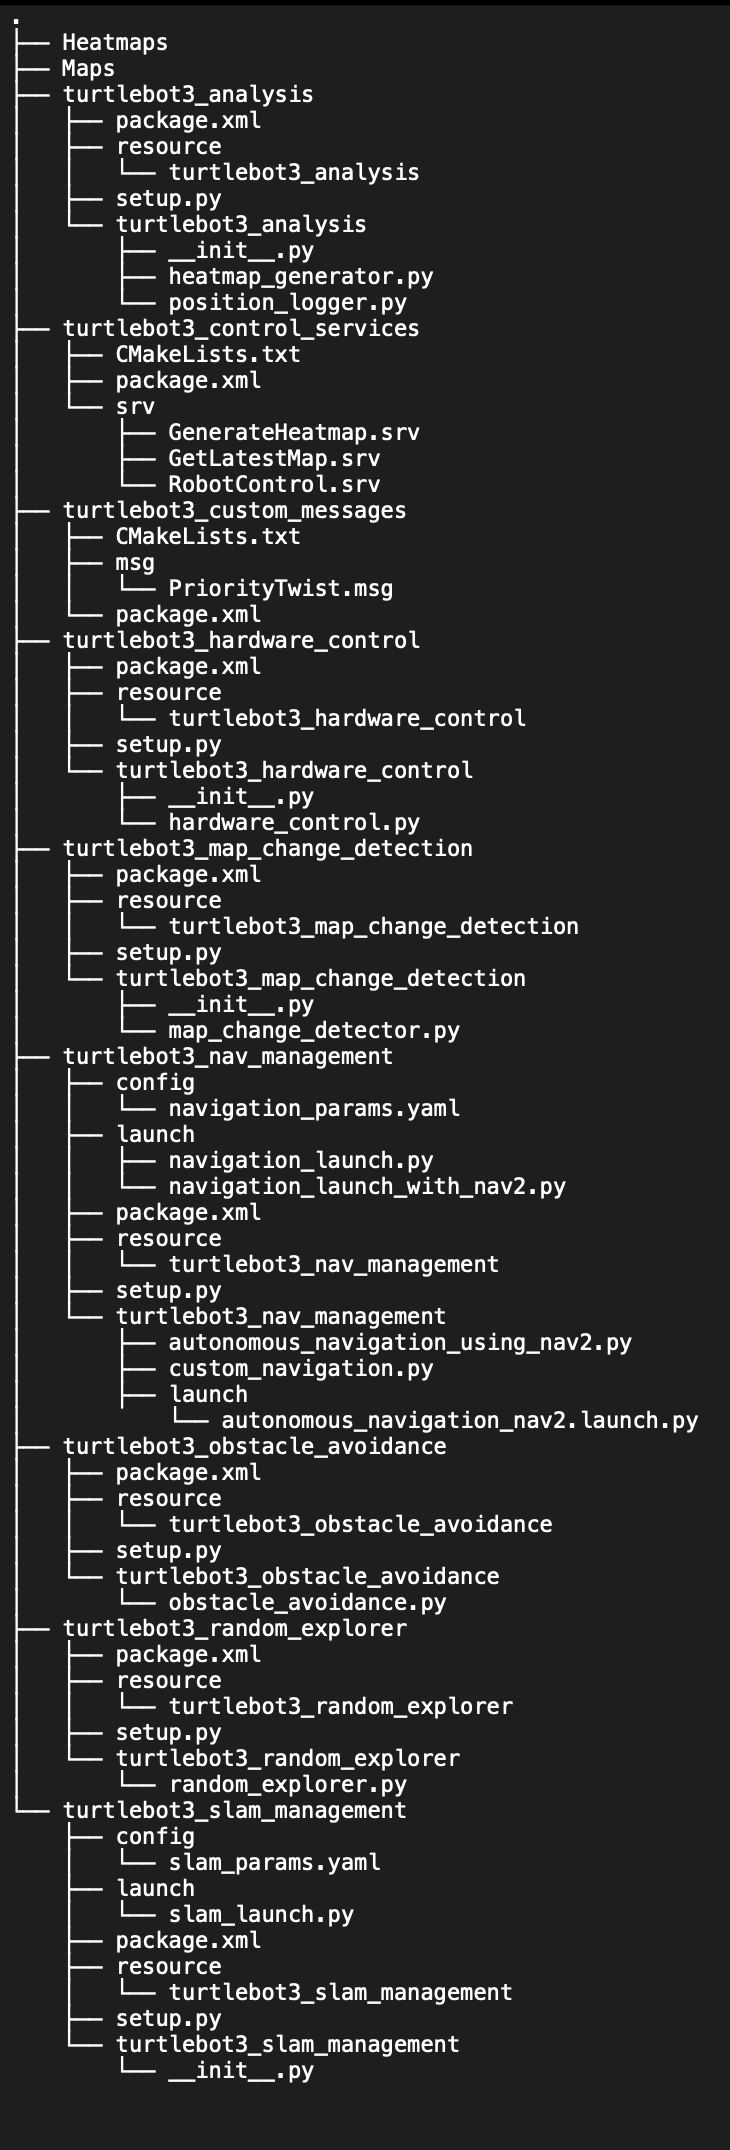
\includegraphics[height=1.0\textheight]{Graphics/tree}
		\caption{Project Directory Tree}
		\label{fig:fig16}
	\end{figure}
	
	\begin{table}[h!]
		\centering
		\begin{tabular}{|c|c|c|}
			\hline
			Coordinate Set & Distance Traveled & Time Used (s) \\
			\hline
			1 & 5.130298 & 27.998535 \\
			1 & 4.869894 & 26.000022 \\
			1 & 5.453286 & 26.000290 \\
			1 & 4.974142 & 26.000858 \\
			1 & 5.387319 & 25.999217 \\
			1 & 5.434525 & 27.999560 \\
			1 & 5.122722 & 26.000072 \\
			1 & 5.448368 & 28.000674 \\
			1 & 5.180251 & 25.999200 \\
			1 & 5.629328 & 29.999985 \\
			1 & 5.352114 & 28.000899 \\
			1 & 5.404368 & 28.000448 \\
			1 & 5.164623 & 25.998860 \\
			1 & 5.398202 & 27.974977 \\
			1 & 5.169252 & 26.025875 \\
			1 & 5.619464 & 29.999127 \\
			1 & 5.327660 & 27.999871 \\
			1 & 5.592663 & 29.760104 \\
			1 & 5.213084 & 26.239961 \\
			\hline
		\end{tabular}
		\caption{Nav2 Data - Coordinate Set 1}
		\label{tab:2}
	\end{table}
	
	
	\begin{table}[h!]
		\centering
		\begin{tabular}{|c|c|c|}
			\hline
			Coordinate Set & Distance Traveled & Time Used (s) \\
			\hline
			2 & 5.311640 & 27.996754 \\
			2 & 4.080332 & 22.000514 \\
			2 & 3.818398 & 19.998617 \\
			2 & 3.761347 & 19.999943 \\
			2 & 3.828356 & 19.999907 \\
			2 & 3.963116 & 22.000073 \\
			2 & 3.884740 & 19.999886 \\
			2 & 4.296424 & 24.000082 \\
			2 & 3.873013 & 20.002518 \\
			2 & 3.839976 & 19.997566 \\
			2 & 3.811117 & 20.000155 \\
			2 & 3.832355 & 20.000026 \\
			2 & 3.866210 & 19.999748 \\
			2 & 3.848264 & 20.001474 \\
			2 & 3.854485 & 19.998312 \\
			2 & 3.844553 & 20.001375 \\
			2 & 3.891537 & 19.998770 \\
			2 & 3.788880 & 20.000184 \\
			2 & 3.852515 & 19.999944 \\
			\hline
		\end{tabular}
		\caption{Nav2 Data - Coordinate Set 2}
		\label{tab:3}
	\end{table}
	
	\begin{table}[h!]
		\centering
		\begin{tabular}{|c|c|c|}
			\hline
			Coordinate Set & Distance Traveled & Time Used (s) \\
			\hline
			3 & 7.566510 & 39.683514 \\
			3 & 4.266853 & 22.316174 \\
			3 & 4.407925 & 22.550062 \\
			3 & 4.395692 & 23.449422 \\
			3 & 4.502186 & 23.999573 \\
			3 & 4.534671 & 23.999918 \\
			3 & 4.417903 & 24.000293 \\
			3 & 4.435943 & 23.999711 \\
			3 & 4.346739 & 24.000350 \\
			3 & 4.278771 & 23.999819 \\
			3 & 4.281278 & 22.000120 \\
			3 & 4.267426 & 21.999995 \\
			3 & 4.340623 & 21.999955 \\
			3 & 4.260607 & 21.999936 \\
			3 & 4.306719 & 22.000231 \\
			3 & 4.243368 & 22.000067 \\
			3 & 4.409689 & 21.999886 \\
			3 & 4.227193 & 22.000825 \\
			3 & 4.373677 & 21.998897 \\
			\hline
		\end{tabular}
		\caption{Nav2 Data - Coordinate Set 3}
		\label{tab:4}
	\end{table}
	
	\begin{table}[h!]
		\centering
		\begin{tabular}{|c|c|c|}
			\hline
			Coordinate Set & Distance Traveled & Time Used (s) \\
			\hline
			4 & 6.377680 & 31.996258 \\
			4 & 4.325679 & 22.000514 \\
			4 & 4.237888 & 19.998617 \\
			4 & 3.761347 & 19.999943 \\
			4 & 4.828356 & 19.999907 \\
			4 & 4.963116 & 22.000073 \\
			4 & 4.884740 & 19.999886 \\
			4 & 4.296424 & 24.000082 \\
			4 & 3.873013 & 20.002518 \\
			4 & 3.839976 & 19.997566 \\
			4 & 3.811117 & 20.000155 \\
			4 & 3.832355 & 20.000026 \\
			4 & 3.866210 & 19.999748 \\
			4 & 3.848264 & 20.001474 \\
			4 & 3.854485 & 19.998312 \\
			4 & 3.844553 & 20.001375 \\
			4 & 3.891537 & 19.998770 \\
			4 & 3.788880 & 20.000184 \\
			4 & 3.852515 & 19.999944 \\
			\hline
		\end{tabular}
		\caption{Nav2 Data - Coordinate Set 4}
		\label{tab:5}
	\end{table}
	
	

	
	% Eidesstattliche Erklärung
	%!TEX root = ../template.tex
\chapter*{Eigenständigkeitserklärung}
\addcontentsline{toc}{chapter}{Eigenständigkeitserklärung} % fügt Erklärung als Eintrag zum Inhaltsverzeichnis (toc) auf Kapitelebene hinzu.
Hiermit versichere ich, dass die vorliegende Masterarbeit mit dem Titel \textit{Layering in Autonomous Robotics: Modular Design and Implementation on the Turtlebot3 Platform using ROS2. } selbstständig verfasst worden ist, dass keine anderen Quellen und Hilfsmittel als die angegebenen benutzt worden sind und dass die Stellen der Arbeit, die anderen Werken -- auch elektronischen Medien -- dem Wortlaut oder Sinn nach entnommen wurden, auf jeden Fall unter Angabe der Quelle als Entlehnung kenntlich gemacht worden sind.

Ich erkläre mich mit einem Abgleich der Arbeit mit anderen Texten zwecks Auffindung von Übereinstimmungen sowie mit einer zu diesem Zweck vorzunehmenden Speicherung der Arbeit in eine Datenbank einverstanden.


\vspace*{2cm}

\begin{minipage}{0.5\textwidth}
  \begin{flushleft} \large
    \underline{\hspace{6cm}} \\
    {\footnotesize (Ort, Datum)}
  \end{flushleft}
\end{minipage}
~
\begin{minipage}{0.5\textwidth}
  \begin{flushright} \large
    \underline{\hspace{6cm}} \\
    {\footnotesize (Unterschrift)}
  \end{flushright}
\end{minipage}\\[0.5cm]
\end{document}
